% relaxation_criteria.tex  -- revised

\documentclass[12pt]{article}
\usepackage[margin=1.1in]{geometry}
\usepackage{amsmath,amssymb}
\usepackage{graphicx}
\usepackage{natbib}
\usepackage{booktabs}
\usepackage{multirow}
\usepackage{hyperref}
\usepackage{xcolor}
\usepackage{array}
\usepackage{float}
\usepackage{caption}
\usepackage{subcaption}
\usepackage{setspace}
\usepackage{parskip}
\usepackage{microtype}
\usepackage{placeins}   % \FloatBarrier

\setstretch{1.15}
\captionsetup{font=small, labelfont=bf}
\bibliographystyle{aasjournal}

% Shorthand
\newcommand{\Mfive}{M_{500c}}
\newcommand{\Rfive}{R_{500c}}
\newcommand{\Rtwo}{R_{200m}}
\newcommand{\Lx}{L_{\rm X}}
\newcommand{\Tsz}{Y_{\rm SZ}}
\newcommand{\Kcore}{K_{\rm core}}
\newcommand{\TPI}{\mathrm{TPI}}
\newcommand{\deltai}{\delta_1}
\newcommand{\deltaii}{\delta_2}
\newcommand{\deltaiii}{\delta_3}
\newcommand{\deltaiv}{\delta_4}
\newcommand{\kevcm}{{\rm keV\,cm^2}}
\newcommand{\Msun}{M_\odot}

%-----------------------------------------------------------------------
\title{\textbf{Relaxation Criteria Beyond Dark Matter Statistics}}
\date{\today}

\begin{document}
\maketitle

%-----------------------------------------------------------------------
\begin{abstract}
Galaxy cluster relaxation state is central to cluster cosmology, influencing mass
calibration biases, intracluster medium (ICM) thermodynamics, and the reliability of
scaling relations.  We present a systematic, multi-criterion analysis of relaxation for
9{,}985 galaxy clusters at $z=0$ drawn from the Frontier-E HACC hydrodynamical
simulation, spanning a mass range $5\times10^{13}$--$10^{15}\,h^{-1}\Msun$.  We define
four complementary criteria probing distinct physical scales: $\deltai$, the dark matter
(DM) center-of-mass offset normalised to $R_{200m}$; $\deltaii$, the DM--gas centroid
separation normalised to $R_{500c}$; $\deltaiii$, the core entropy $\Kcore$ with a
cool-core threshold of $150\,\kevcm$ \citep{hudson2010}; and $\deltaiv$, the Thermal
Profile Indicator (TPI), combining core electron density and core temperature ratio.

Using DM relaxation ($\deltai$) as a structural baseline, we demonstrate that the
secondary criteria probe physically distinct radial regimes: $\deltaii$ discriminates
at $0.3$--$0.7\,\Rfive$ via bulk sloshing and gas displacement, while $\deltaiii$ and
$\deltaiv$ discriminate sharply below $0.15\,\Rfive$, tracing core thermodynamic state.
Cool-core clusters (R3) within the DM-relaxed subsample show one-to-two order-of-magnitude
central X-ray luminosity enhancements, steep density cusps, and entropy profiles $2$--$3$
times lower than their non-cool-core counterparts at $r < 0.05\,\Rfive$.
These differences are entirely absent at $r > 0.15\,\Rfive$, establishing a clean
physical scale separation between structural and thermodynamic relaxation.
Cool-core clusters are elevated in $L_X$ at fixed spectroscopic temperature by up to a
factor of $\sim$3, and show $\sim$30\% lower scatter in the $Y_{\rm SZ}$--$M_{500c}$
relation, confirming the importance of relaxation-state selection for precision cluster
cosmology.  The TPI criterion, which independently tracks the density and temperature
channels of cool-core formation, reveals a distinct population of clusters with strong
temperature drops but moderate core density, providing finer-grained thermodynamic
information than core entropy alone.
\end{abstract}

%-----------------------------------------------------------------------
\section{Introduction}
\label{sec:intro}

Galaxy clusters are the most massive collapsed objects in the universe and powerful
cosmological probes.  Their number counts as a function of mass and redshift are
exquisitely sensitive to the matter power spectrum and dark energy equation of state
\citep{mantz2015}.  However, realising this potential requires accurate mass calibration,
which in turn depends on the dynamical state of individual clusters.
Disturbed clusters in the process of merging have systematically biased hydrostatic
equilibrium estimates \citep{biffi2016,rasia2013}, enhanced non-thermal pressure support
\citep{nagai2007}, and scatter in X-ray and Sunyaev-Zel'dovich (SZ) scaling relations
\citep{kravtsov2006}.

Cluster relaxation state is not a single, well-defined quantity.  Different observational
tracers --- X-ray morphological asymmetry, centroid shifts, power ratios, the presence
of a cool core, the existence of a radio mini-halo --- probe different physical scales
and different physical processes.  A cluster may appear dynamically relaxed at large
radii while its core undergoes active AGN feedback or sloshing \citep{markevitch2007,
zuhone2010}.  Conversely, a cluster with a smooth outer morphology may be experiencing
a minor merger that has not yet disrupted its cool core.
These distinctions matter not just for mass calibration but for understanding ICM physics:
the cool-core/non-cool-core dichotomy reflects different thermal histories, entropy
injection histories, and feedback efficiencies \citep{burns2008,gitti2012}.

In observational samples, relaxation state is often assessed through a single scalar
metric: the power ratio \citep{poole2007}, the centroid shift \citep{cassano2010},
or the central cooling time \citep{hudson2010}.  Each has its own observational
systematics, and they are not always mutually consistent.  Hydrodynamical simulations
offer a ground-truth comparison: they provide simultaneous access to the DM structural
state, the gas morphological state, and the full thermodynamic profiles, enabling a
systematic multi-criterion classification.

In this work we apply four complementary relaxation criteria to 9{,}985 galaxy clusters
from the Frontier-E HACC hydrodynamical simulation \citep{hacc2016} at $z = 0$.
The DM center-of-mass offset ($\deltai$) serves as a structural baseline, and we
characterise how the secondary criteria ($\deltaii$, $\deltaiii$, $\deltaiv$) each
reveal distinct ICM signatures at characteristic radial scales, as traced by stacked
profiles, ratio profiles, scaling relations, and extreme representatives.

The paper is organised as follows.
Section~\ref{sec:data} describes the simulation and data products.
Section~\ref{sec:criteria} defines the four relaxation criteria.
Section~\ref{sec:profiles} analyses ICM profiles stratified by relaxation state,
using $\deltai$ as the structural baseline.
Section~\ref{sec:scaling} examines cluster scaling relations.
Section~\ref{sec:thermo} discusses core thermodynamic indicators.
Section~\ref{sec:extreme} presents extreme unrelaxed systems.
Section~\ref{sec:discuss} discusses astrophysical implications.
Section~\ref{sec:conclusions} summarises our findings.
Cross-classification statistics and the TPI diagnostic are provided in the Appendix.

%-----------------------------------------------------------------------
\section{Simulation and Data}
\label{sec:data}

\subsection{The Frontier-E Simulation}

Frontier-E is a large-volume full-physics hydrodynamical simulation run with the
Hardware/Hybrid Accelerated Cosmology Code \citep[HACC;][]{hacc2016}.  The simulation
adopts a flat $\Lambda$CDM cosmology consistent with Planck 2018 results \citep{planck2018}:
$H_0 = 67.66\,{\rm km\,s^{-1}\,Mpc^{-1}}$, $\Omega_m = 0.3096$, $\Omega_b = 0.04897$.
The hydrodynamics include radiative cooling, star formation, stellar feedback, and
AGN feedback via a kinetic-mode prescription.  HACC's PM+PP gravitational solver and
spectral mesh gas solver provide high spatial dynamic range, enabling accurate treatment
of both cluster outskirts and dense cores.

\subsection{Halo Catalog and Profile Data}

We analyse 10{,}000 halos extracted at $z=0$ using the Spherical Overdensity (SO) halo
finder with overdensity threshold $\Delta = 500c$ relative to the critical density.
After removing objects with non-finite values in any of the quantities required for our
criteria, the final sample contains $N = 9{,}985$ halos spanning
$5\times10^{13}$--$10^{15}\,h^{-1}\Msun$ in $M_{500c}$.

Each halo has 51 logarithmically spaced radial profile bins from the center to
$\sim 2.5\,\Rfive$, providing density, temperature, entropy, pressure, X-ray emissivity,
radial velocity, gas fraction, metallicity, and enclosed mass profiles.
The catalog provides over 80 scalar properties per halo including X-ray luminosities,
spectroscopic temperatures, the SZ Compton-$y$ parameter, DM concentration, core electron
density, core entropy, and AGN properties.  Key quantities used in this work are
summarised in Table~\ref{tab:catalog_cols}.

\begin{table}[htbp]
\centering
\caption{Key catalog quantities used in this work.}
\label{tab:catalog_cols}
\begin{tabular}{lll}
\toprule
Column & Description & Units \\
\midrule
\texttt{fof\_halo\_mass}          & Friends-of-friends total mass              & $h^{-1}\Msun$    \\
\texttt{sod\_halo\_M500c}         & SO mass within $R_{500c}$                  & $h^{-1}\Msun$    \\
\texttt{sod\_halo\_radius}        & $R_{500c}$ radius                          & $h^{-1}$Mpc      \\
\texttt{sod\_halo\_cdelta}        & NFW concentration $c_{500}$                & ---              \\
\texttt{sod\_halo\_core\_entropy} & Core specific entropy $\Kcore$             & $\kevcm$         \\
\texttt{sod\_halo\_core\_ne}      & Core electron number density               & cm$^{-3}$        \\
\texttt{sod\_halo\_T500c}         & Spectroscopic temperature in $R_{500c}$    & keV              \\
\texttt{sod\_halo\_T500cBoloEx}   & Core-excised bolometric temperature        & keV              \\
\texttt{sod\_halo\_L500cBolo}     & Bolometric $L_X$ within $R_{500c}$        & $h^{-2}$erg/s    \\
\texttt{sod\_halo\_Y500c}         & Integrated SZ parameter $Y_{500c}$        & $h^{-2}$Mpc$^2$  \\
\bottomrule
\end{tabular}
\end{table}

\FloatBarrier
%-----------------------------------------------------------------------
\section{Relaxation Criteria}
\label{sec:criteria}

We define four relaxation criteria probing distinct physical scales.
The first two characterise the dynamical state of the DM and gas at intermediate-to-large
radii; the latter two probe the ICM thermodynamic state of the cluster core.
All four criteria and their thresholds are summarised in Table~\ref{tab:criteria}.

\begin{table*}[htbp]
\centering
\caption{Relaxation criteria: definitions, physical motivation, observational analogues, and thresholds.}
\label{tab:criteria}
\begin{tabular}{p{1.4cm} p{5.2cm} p{3.0cm} p{3.5cm} p{1.4cm} p{1.6cm}}
\toprule
Criterion & Formula & Physical Quantity & Observational Proxy & Threshold & Relaxed if \\
\midrule
$\deltai$
  & $|\mathbf{r}_{\rm COM}^{\rm FoF} - \mathbf{r}_{\rm min}^{\rm FoF}| /\, R_{200m}$
  & DM structural offset
  & X-ray centroid shift
  & 0.07
  & $\deltai < 0.07$ \\[6pt]
$\deltaii$
  & $|\mathbf{r}_{\rm COM}^{\rm DM} - \mathbf{r}_{\rm COM}^{\rm gas}| /\, R_{500c}$
  & DM--gas centroid offset
  & Optical--X-ray peak offset
  & 0.07
  & $\deltaii < 0.07$ \\[6pt]
$\deltaiii$
  & $\Kcore\;[\kevcm]$
  & Core specific entropy
  & X-ray core cooling time
  & 150
  & $\Kcore < 150$ \\[6pt]
$\deltaiv$
  & $z[\ln n_{e,\rm core}] + z[\ln(T_{\rm BoloEx}/T_{500c})]$
  & Composite thermal state
  & Core imaging + spectroscopy
  & 0
  & $\TPI > 0$ \\
\bottomrule
\end{tabular}
\par\smallskip
\raggedright\footnotesize
\emph{Note.} $z[x]$ denotes the robust $z$-score, $z[x]=(x-\mathrm{median}[x])/(1.4826\,\mathrm{MAD}[x])$,
computed across the full sample.
The threshold $\Kcore < 150\,\kevcm$ for cool-core classification follows \citet{hudson2010},
derived from a complete X-ray flux-limited sample of nearby clusters.
Abbreviation: MAD = median absolute deviation.
\end{table*}

\subsection{\texorpdfstring{$\deltai$}{delta1}: Dark Matter Structural Offset}

The first criterion quantifies the offset between the friends-of-friends (FoF) halo
center of mass and the position of the DM potential minimum:
\begin{equation}
  \deltai = \frac{|\mathbf{r}_{\rm COM}^{\rm FoF} - \mathbf{r}_{\rm min}^{\rm FoF}|}{R_{200m}}.
\end{equation}
A large $\deltai$ indicates that the DM halo has not yet relaxed following a merger:
its mass distribution is globally asymmetric, with a substantial off-center substructure
or secondary clump pulling the center of mass away from the potential minimum.
We adopt the threshold $\deltai < 0.07$ to define DM-dynamically relaxed halos (R1),
consistent with DM-only simulation studies \citep{neto2007}.
This criterion is sensitive to major mergers and large-scale structural disturbances
at $r \gtrsim 0.3\,\Rtwo$.  Of the 9{,}985 halos, 4{,}640 (46.5\%) satisfy R1.

\subsection{\texorpdfstring{$\deltaii$}{delta2}: DM--Gas Centroid Separation}

The second criterion measures the separation between the DM center of mass and the gas
center of mass, normalised to $\Rfive$:
\begin{equation}
  \deltaii = \frac{|\mathbf{r}_{\rm COM}^{\rm DM} - \mathbf{r}_{\rm COM}^{\rm gas}|}{R_{500c}}.
\end{equation}
Mergers, sloshing episodes, and ram-pressure stripping can displace the gas component
relative to the DM skeleton.  This criterion complements $\deltai$: a cluster may have a
well-relaxed DM structure while its gas has been displaced by a recent interaction.
We use the threshold $\deltaii < 0.07$ (criterion R2).  Within DM-relaxed halos,
4{,}198 of 4{,}640 (90.5\%) also satisfy R2, indicating that most DM-relaxed clusters
maintain coherent DM--gas morphology; the 442 exceptions are candidates for gas-sloshing
in an otherwise settled gravitational potential.
Observationally, $\deltaii$ is analogous to the offset between optical/lensing peak and
X-ray centroid \citep{cassano2010}.

\subsection{\texorpdfstring{$\deltaiii$}{delta3}: Core Entropy}

The core specific entropy,
\begin{equation}
  \Kcore = T_e\,n_e^{-2/3}\quad [\kevcm],
\end{equation}
is a direct thermodynamic tracer of the ICM cooling and heating history.
Cool-core clusters develop low-entropy central gas through efficient radiative cooling,
which creates steep central temperature drops and luminous X-ray cores.
Non-cool-core clusters have elevated core entropy, indicating that their cores have been
heated by AGN feedback, merger-driven shocks, or conduction.
Following \citet{hudson2010}, we adopt $\Kcore < 150\,\kevcm$ as the cool-core threshold
(criterion R3).  In our catalog, $\Kcore$ spans 64--347\,$\kevcm$ (median $\approx 150$),
providing excellent discriminating power across the threshold.
Of the 9{,}985 halos, 4{,}997 (50.0\%) are classified as cool-core by R3.

\subsection{\texorpdfstring{$\deltaiv$}{delta4}: Thermal Profile Indicator (TPI)}
\label{sec:tpi_def}

While $\Kcore$ combines density and temperature in a single scalar, different astrophysical
processes can produce similar entropy values through different paths.  We define a composite
fourth criterion that retains information from the two independent observational channels of
X-ray imaging and spectroscopy separately:
\begin{equation}
  \TPI = z[\ln n_{e,\rm core}] + z[\ln(T_{\rm BoloEx}/T_{500c})],
  \label{eq:tpi}
\end{equation}
where $T_{\rm BoloEx}$ is the bolometric core-excised temperature and $z[x]$ is the
robust $z$-score (Table~\ref{tab:criteria}).
A positive TPI indicates above-median core electron density \emph{and} an above-median
temperature ratio $T_{\rm BoloEx}/T_{500c} > 1$ --- the spectroscopic cool-core signature,
where the core region is cooler than the bulk ICM.  We classify halos with $\TPI > 0$
as cool-core (criterion R4); 5{,}344 halos (53.5\%) satisfy R4.

The key distinction from $\Kcore$ is that TPI is sensitive to the \emph{co-occurrence}
of high density and a temperature drop.  This resolves cases where $K_{\rm core}$ is
degenerate: a cluster can have low entropy from high density alone (without a temperature
drop), or from a strong temperature decrease at moderate density.
Full population concordance statistics between all four criteria are provided in
Appendix~\ref{app:concordance}.

\FloatBarrier
%-----------------------------------------------------------------------
\section{Radial Profile Analysis}
\label{sec:profiles}

\subsection{DM Relaxation as a Structural Baseline}
\label{sec:profiles_dm}

We use the DM relaxation criterion ($\deltai$, R1) as a structural baseline dividing the
full halo sample into dynamically settled (R1) and dynamically disturbed ($\lnot$R1)
subsamples.  The contrast between R1 and $\lnot$R1 halos sets the envelope of
differentiation driven purely by DM-scale disturbances.  Within this baseline, the
secondary criteria R2, R3, and R4 reveal further stratification, each sensitive to
a different physical regime.

Figure~\ref{fig:profiles_comprehensive} is the central result of this work.
It shows stacked median profiles and their 16th--84th percentile scatter bands for
five ICM quantities: enclosed mass, gas electron density $n_e$, specific entropy $K$,
thermal pressure $P$, and bolometric X-ray luminosity $L_X$.  The four columns compare:
(1) R1 vs.\ $\lnot$R1 (the DM structural baseline); (2) R1$\cap$R2 vs.\ R1$\cap\lnot$R2
(DM--gas morphological criterion within DM-relaxed halos); (3) R1$\cap$R3 vs.\
R1$\cap\lnot$R3 (core entropy criterion within DM-relaxed halos); and (4) R1$\cap$R4
vs.\ R1$\cap\lnot$R4 (TPI criterion within DM-relaxed halos).

\begin{figure*}[htbp]
  \centering
  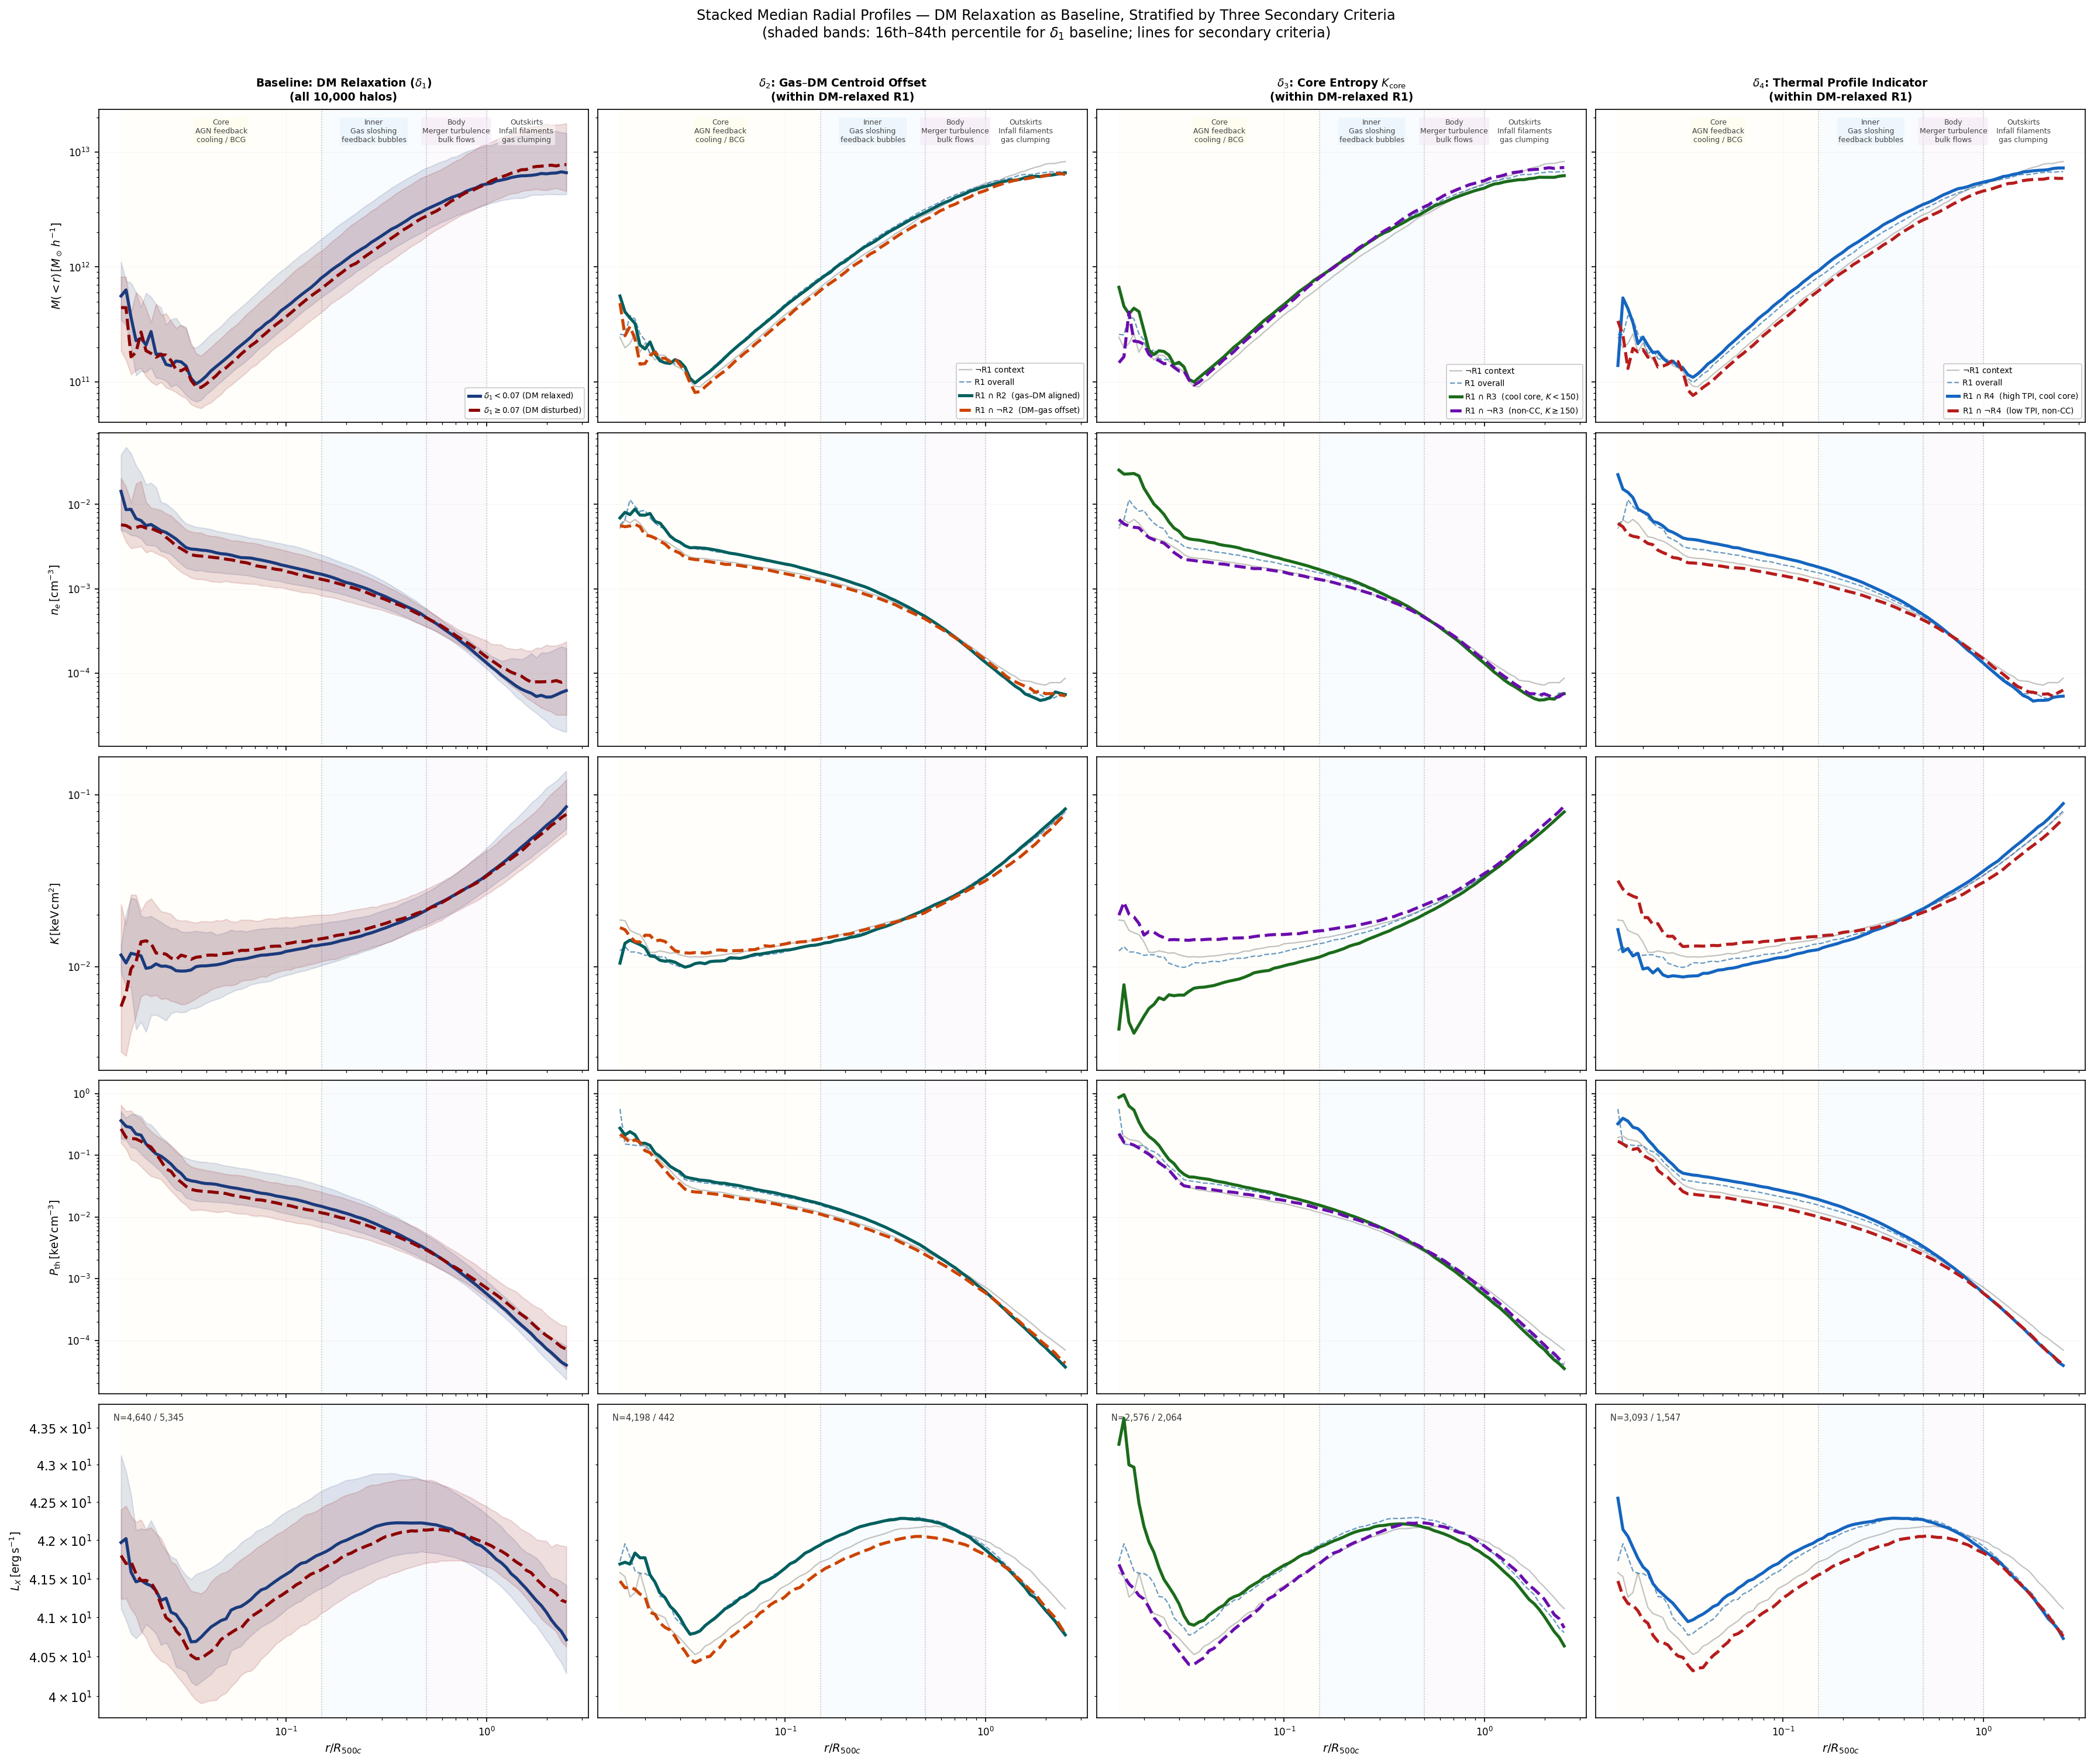
\includegraphics[width=\textwidth]{phase6_stacked_profiles_comprehensive.png}
  \caption{Stacked median radial profiles for five ICM quantities stratified by
    relaxation criterion.
    \emph{Columns, left to right:} (1) All halos, split by DM relaxation (R1 vs.\ $\lnot$R1).
    (2) DM-relaxed halos split by DM--gas coherence (R1$\cap$R2 vs.\ R1$\cap\lnot$R2).
    (3) DM-relaxed halos split by core entropy (R1$\cap$R3 vs.\ R1$\cap\lnot$R3).
    (4) DM-relaxed halos split by TPI (R1$\cap$R4 vs.\ R1$\cap\lnot$R4).
    \emph{Rows, top to bottom:} enclosed mass, gas electron density, specific entropy,
    thermal pressure, bolometric X-ray luminosity.
    Shaded bands show 16th--84th percentile range.
    Thin lines in columns~2--4 show the R1 (navy dashed) and $\lnot$R1 (gray solid)
    reference profiles for scale.
    Vertical background shading indicates four radial zones: Core ($r < 0.15\,\Rfive$,
    yellow), Inner ($0.15$--$0.5\,\Rfive$, pale blue), Body ($0.5$--$1.0\,\Rfive$,
    pale purple), Outskirts ($r > 1.0\,\Rfive$, white).}
  \label{fig:profiles_comprehensive}
\end{figure*}

\paragraph{Column 1: DM relaxation (R1 vs.\ $\lnot$R1) --- the baseline.}
DM-disturbed clusters show: (i) modestly elevated enclosed mass at $r > 0.5\,\Rfive$
from infalling substructure; (ii) slightly higher gas density at intermediate radii
($0.3$--$0.7\,\Rfive$), reflecting enhanced gas filaments and infalling blobs;
(iii) elevated entropy throughout, indicating a less thermodynamically evolved state;
(iv) flatter pressure profiles; and (v) modestly suppressed outskirt X-ray luminosity.
These DM-scale differences are \emph{moderate} --- the ICM at intermediate and large radii
is mildly perturbed, but the core profiles of R1 and $\lnot$R1 halos overlap substantially.
This baseline establishes the maximum differentiation that DM structure alone can provide.

\paragraph{Column 2: DM--gas coherence (R2) within DM-relaxed halos.}
Within DM-relaxed halos, the 442 R1$\cap\lnot$R2 halos (DM-settled but gas-displaced)
show elevated gas density and pressure at $0.3$--$0.7\,\Rfive$ compared to the 4{,}198
R1$\cap$R2 halos.  This is the profile signature of gas sloshing: the gas centroid is
displaced from the potential minimum, creating a one-sided density and pressure enhancement
at intermediate radii.  Crucially, the core profiles ($r < 0.15\,\Rfive$) are nearly
identical for R2 and $\lnot$R2 groups within R1, confirming that $\deltaii$ is sensitive
to intermediate-radius gas dynamics rather than core thermodynamics.

\paragraph{Column 3: Core entropy (R3) within DM-relaxed halos.}
The core entropy criterion produces the most dramatic profile differentiation.
Within DM-relaxed halos, the 2{,}576 cool-core clusters (R1$\cap$R3) show:
(i) steeply rising central electron density ($n_e \propto r^{-1}$ at small $r$);
(ii) central entropy $2$--$3\times$ lower than non-cool-core clusters at $r < 0.05\,\Rfive$;
(iii) a pronounced central pressure peak; and
(iv) X-ray luminosity enhanced by nearly an order of magnitude in the innermost bin
  relative to the 2{,}064 R1$\cap\lnot$R3 clusters.
This is the canonical ICM cool-core signature \citep{vikhlinin2006}: efficient cooling
drives rapid central density growth, amplifying the X-ray surface brightness concentration.
Outside $0.15\,\Rfive$, the R3 and $\lnot$R3 profiles converge completely --- cool-core
differences are confined entirely to the cluster core.

\paragraph{Column 4: TPI (R4) within DM-relaxed halos.}
The TPI criterion produces qualitatively similar profile differences to R3 but with a
more gradual transition.  The 3{,}093 R1$\cap$R4 clusters have elevated core density and
pressure, but with somewhat less extreme values than R1$\cap$R3.  TPI requires that
\emph{both} the density enhancement and the temperature drop exceed their sample medians,
so clusters with high density but a modest temperature ratio (which R3 classifies as
cool-core) score modestly on TPI.  Consequently, the TPI criterion is more conservative
in identifying the strongest cool cores but more sensitive to systems where the temperature
drop is the dominant cool-core signal.

\subsection{Criterion Discrimination by Radius}
\label{sec:profiles_ratio}

Figure~\ref{fig:ratios} quantifies the radial scale on which each secondary criterion
discriminates, showing $\log_{10}(\text{R1}\cap R_x / \text{R1}\cap\lnot R_x)$ for
$x = 2, 3, 4$ (rows) and all five profiles (columns).  A positive value means the
criterion-relaxed subgroup has higher profile values; negative means lower.

\begin{figure*}[htbp]
  \centering
  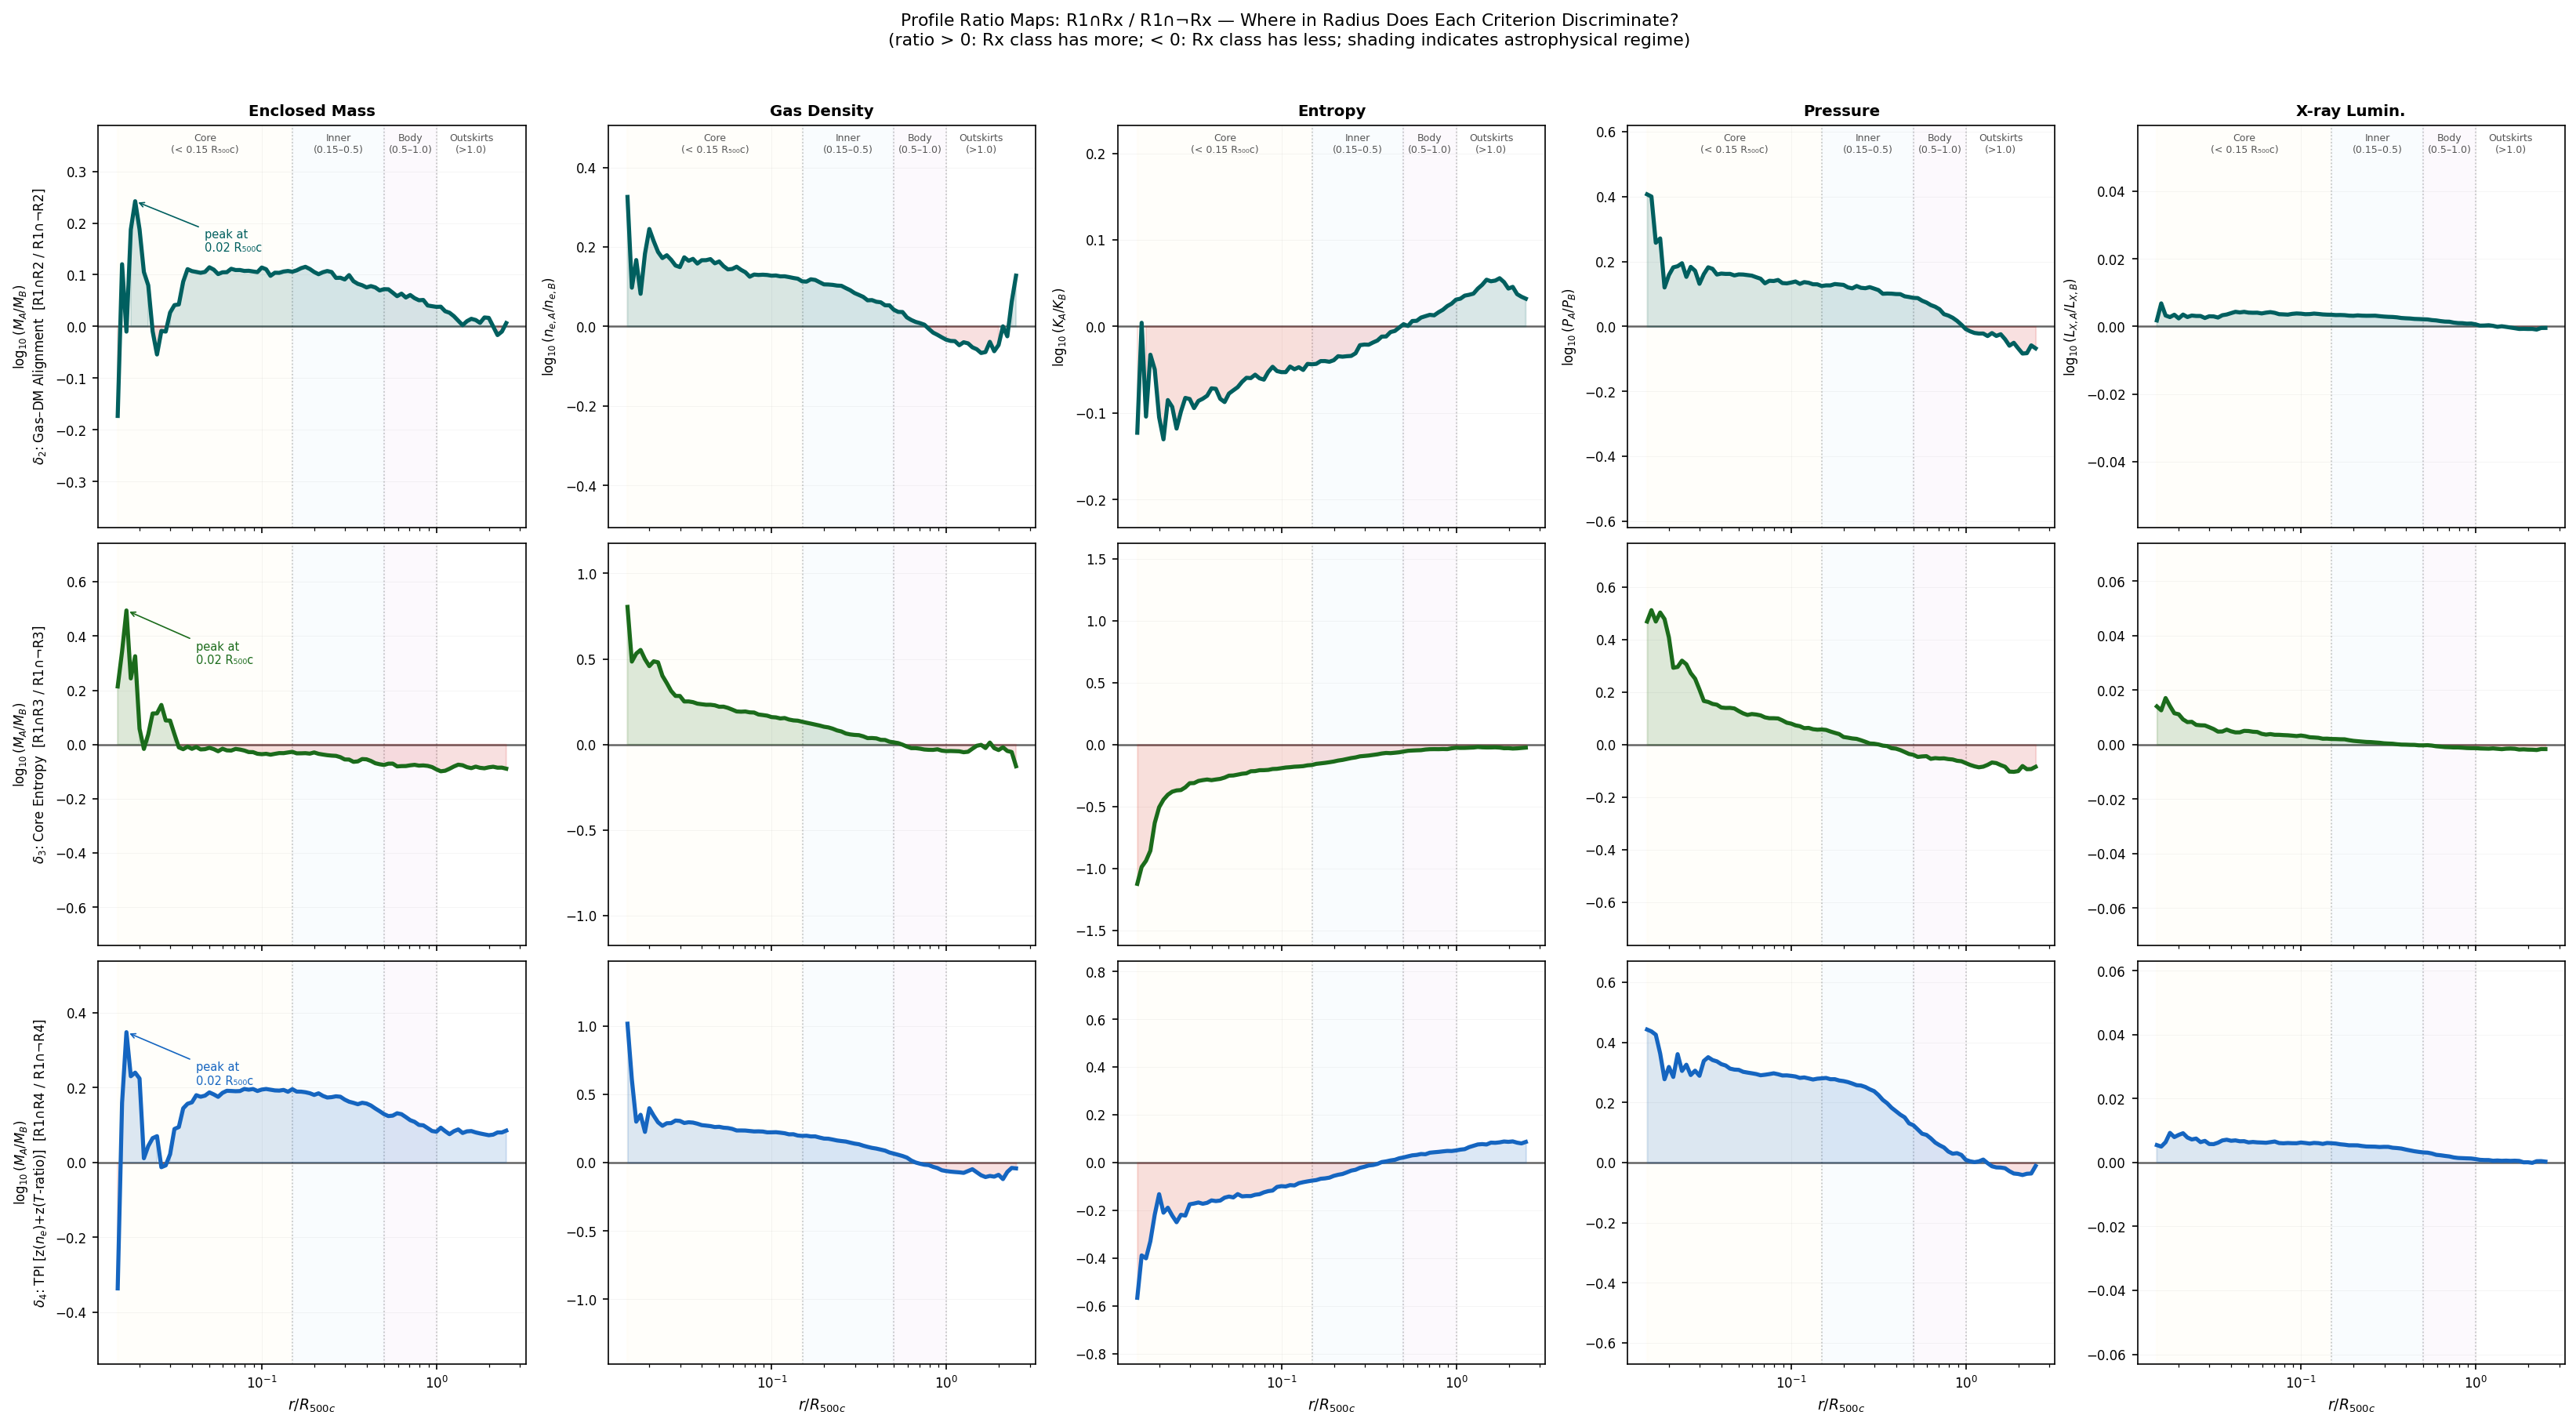
\includegraphics[width=\textwidth]{phase6_ratio_profiles.png}
  \caption{Log ratio profiles $\log_{10}(\text{R1}\cap R_x\;/\;\text{R1}\cap\lnot R_x)$
    for the three secondary criteria ($x=2,\,3,\,4$; rows) and five ICM quantities
    (columns).  Positive values indicate higher profiles for the criterion-relaxed
    sub-sample; negative values indicate lower.  Shaded bands show 16th--84th percentile
    scatter.  Vertical dashed lines mark the radial zone boundaries at $0.15$ and
    $0.5\,\Rfive$.  The peak location of each ratio curve identifies the radial scale
    at which that criterion most powerfully discriminates within DM-relaxed halos.}
  \label{fig:ratios}
\end{figure*}

The top row ($\deltaii$, DM--gas coherence) shows ratio peaks between $0.3$ and
$0.7\,\Rfive$ in gas density and pressure --- the inner body of the cluster, where
sloshing motions and off-axis merger-driven redistribution are most active.  The ratio
approaches unity in both the core ($r < 0.15\,\Rfive$) and the outskirts
($r > \Rfive$), confirming that $\deltaii$ discriminates \emph{only} at intermediate scales.

The middle row ($\deltaiii$, core entropy) and bottom row ($\deltaiv$, TPI) both show
sharply peaked ratios inside $0.15\,\Rfive$, with the largest signals in entropy,
electron density, and X-ray luminosity.  The X-ray luminosity ratio reaches
$\sim$0.5--0.7 dex in the innermost profile bin --- a factor of 3--5 enhancement
attributable to the luminosity concentration of cool cores.  Both thermodynamic
criteria are entirely insensitive to cluster structure outside the central 15\% of $\Rfive$.

Table~\ref{tab:discrimination} synthesises these findings into a criterion--profile--radius
reference matrix.

\begin{table*}[htbp]
\centering
\caption{Criterion--profile--radius discrimination matrix.}
\label{tab:discrimination}
\begin{tabular}{p{2.0cm} p{3.8cm} p{2.5cm} p{2.8cm} p{4.5cm}}
\toprule
Criterion & Most discriminating profiles & Peak radial zone & Radial scale & Primary astrophysical driver \\
\midrule
$\deltai$ (COM offset)
  & Enclosed mass, gas density
  & Body, Outskirts
  & $0.3$--$1.0\,\Rfive$
  & Major merger, substructure, large-scale accretion \\[4pt]
$\deltaii$ (DM--gas offset)
  & Gas density, pressure
  & Inner--Body
  & $0.3$--$0.7\,\Rfive$
  & Gas sloshing, off-axis merger, ram-pressure displacement \\[4pt]
$\deltaiii$ ($\Kcore$)
  & Entropy, $n_e$, $L_X$
  & Core
  & $r < 0.15\,\Rfive$
  & Radiative cooling history, AGN feedback, core heating \\[4pt]
$\deltaiv$ (TPI)
  & $n_e$, temperature ratio, $L_X$
  & Core
  & $r < 0.15\,\Rfive$
  & Core density peak (X-ray imaging) + temperature drop (spectroscopy) \\
\bottomrule
\end{tabular}
\end{table*}

\FloatBarrier
%-----------------------------------------------------------------------
\section{Particle Morphology and Visual Signatures}
\label{sec:morphology}

The radial profile analysis quantifies \emph{averaged} structural differences between
relaxation sub-classes; particle projections reveal the underlying \emph{visual morphology}.
Figure~\ref{fig:gallery} shows the rank-1 (most extreme) halo from each of the seven
groups studied in Section~\ref{sec:profiles}, rendered in four complementary channels:
dark matter mass, stellar mass, gas mass, and gas temperature.

\begin{figure*}[htbp]
  \centering
  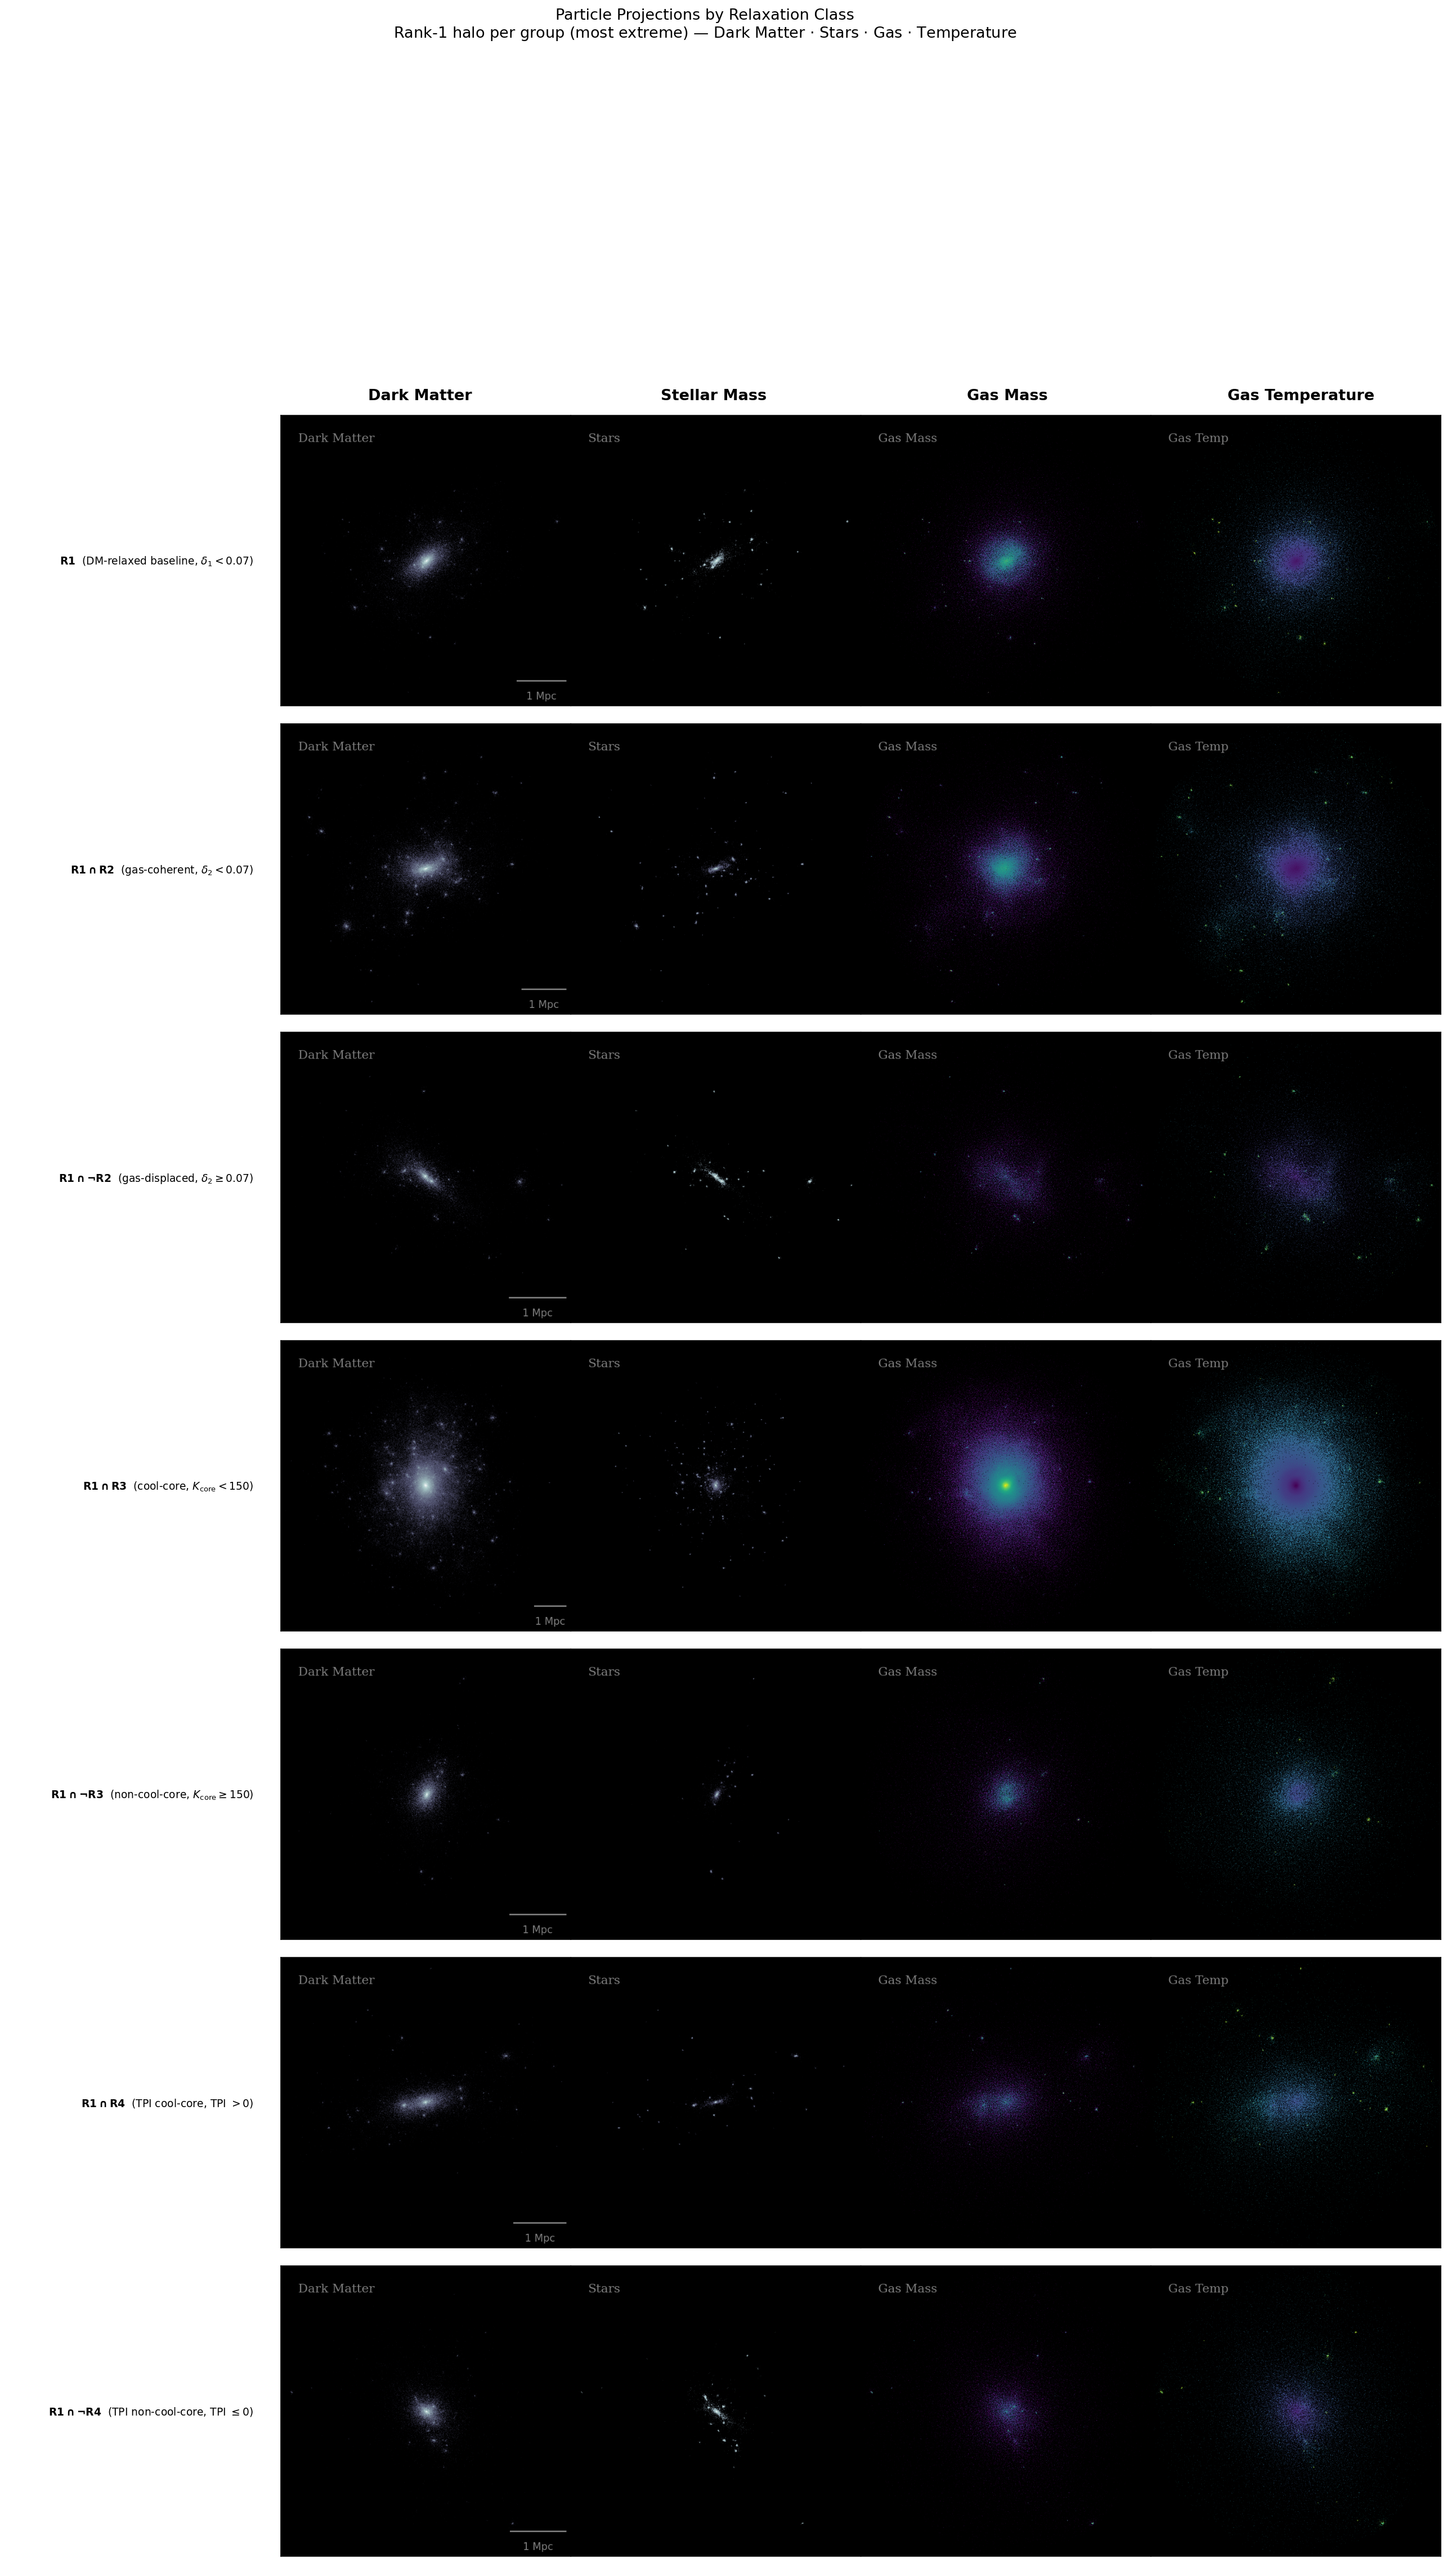
\includegraphics[width=\textwidth]{phase7_particle_gallery.png}
  \caption{Particle projection gallery.  Each row shows the most extreme halo in one
    relaxation sub-class (rank 1 by the group's defining criterion), projected along the
    $z$-axis over a region spanning $2\,R_{200m}$.  Columns show (left to right): dark
    matter mass, stellar mass, gas mass, and gas temperature, using the bone, bone,
    viridis, and reversed viridis colourmaps respectively.  Row labels identify the group
    and its defining threshold.  The R1 baseline shows a typical DM-relaxed cluster;
    subsequent rows demonstrate the range of baryonic structure coexisting with DM
    relaxation.  R1$\cap$R2 halos exhibit centred gas distributions closely tracing the
    DM; R1$\cap\lnot$R2 halos show offset or asymmetric gas cores, a direct visual
    signature of $\deltaii$.  R1$\cap$R3 halos display compact, bright cool cores with
    a central temperature inversion; R1$\cap\lnot$R3 halos have diffuse, isothermal gas.
    The TPI-selected pair ($\deltaiv$) shows analogous contrast in core temperature
    structure.}
  \label{fig:gallery}
\end{figure*}

\FloatBarrier

%-----------------------------------------------------------------------
\section{Scaling Relations}
\label{sec:scaling}

Figure~\ref{fig:scaling} shows the $L_X$--$T$ and $Y_{\rm SZ}$--$M_{500c}$ scaling relations,
with points colour-coded by relaxation class as defined in Appendix~\ref{app:concordance}.

\begin{figure*}[htbp]
  \centering
  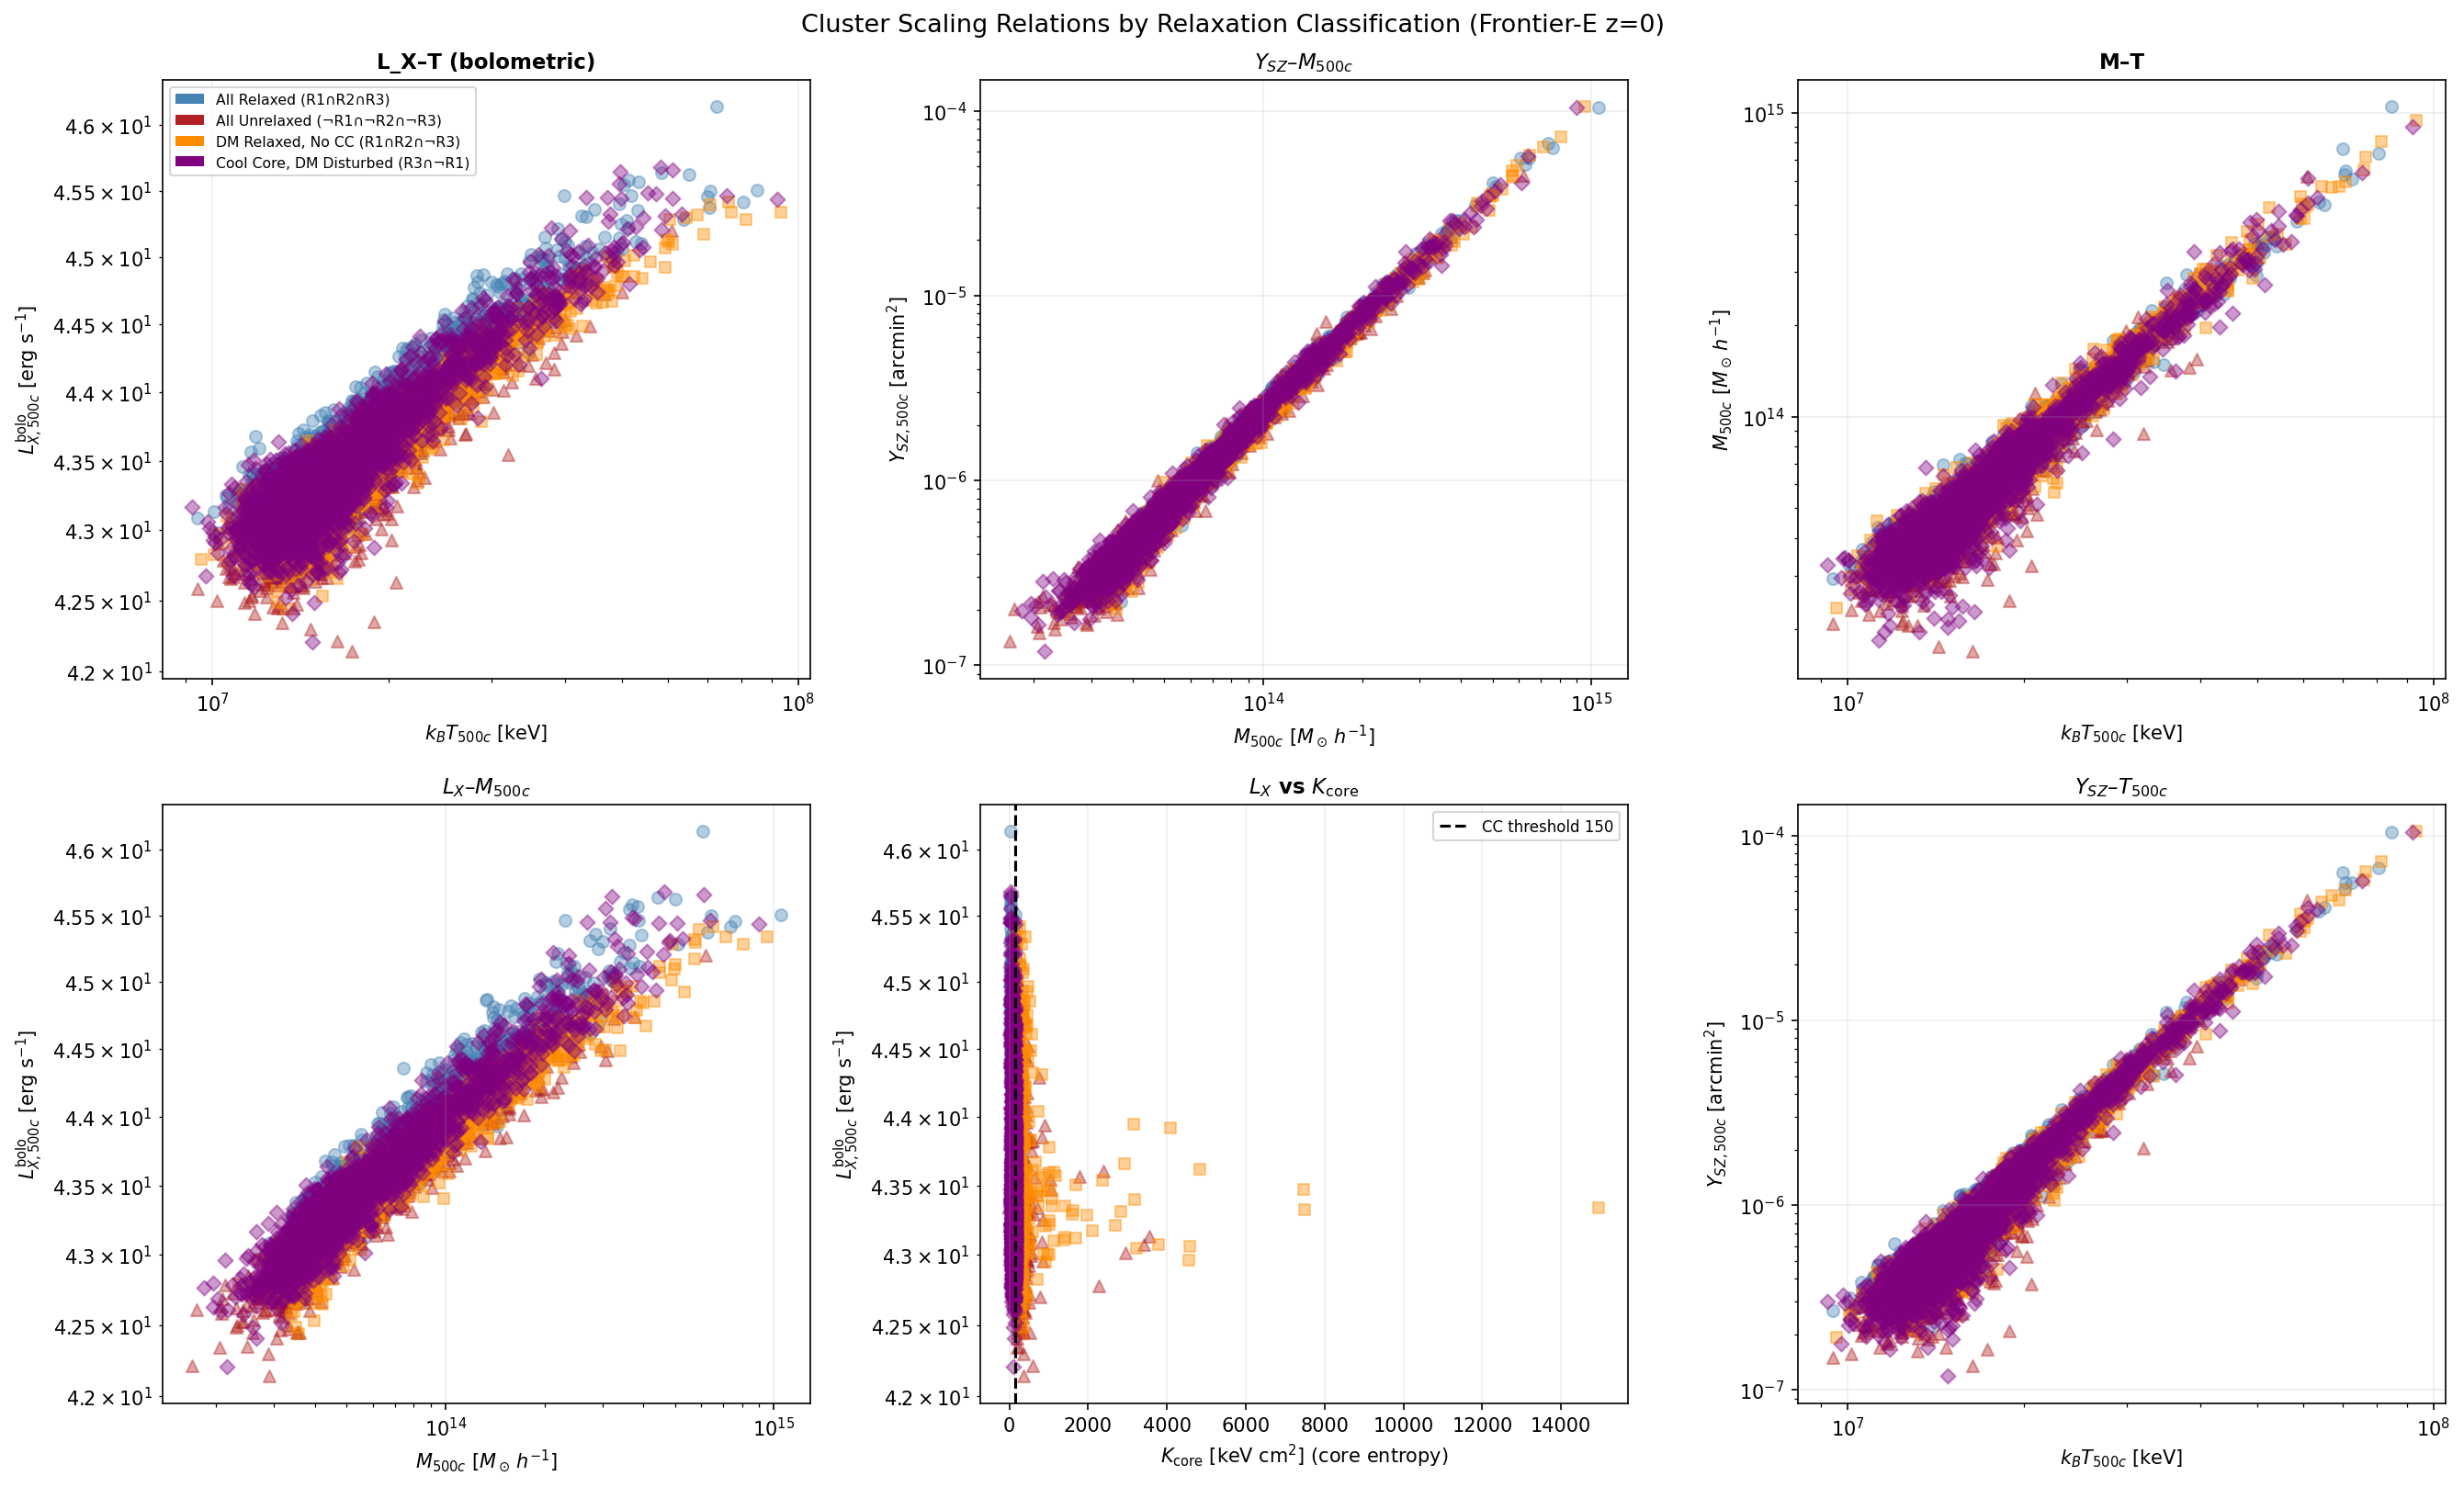
\includegraphics[width=\textwidth]{phase5_scaling_relations.png}
  \caption{Cluster scaling relations colour-coded by relaxation class.
    \emph{Left:} Bolometric X-ray luminosity vs.\ spectroscopic temperature (the $L_X$--$T$
    relation).  \emph{Right:} Integrated SZ parameter $Y_{500c}$ vs.\ $M_{500c}$ (the
    $Y_{\rm SZ}$--$M$ relation).  Relaxation classes: concordant relaxed (blue),
    DM-disturbed cool-core (orange), DM-relaxed/no-cool-core (green), concordant disturbed
    (red); all other halos in grey.  Dashed lines show power-law fits to the full sample.
    Cool-core clusters are elevated in $L_X$ at fixed $T$, while the $Y_{\rm SZ}$--$M$
    relation is tighter for relaxed clusters.}
  \label{fig:scaling}
\end{figure*}

\paragraph{$L_X$--$T$ relation.}
Cool-core populations (concordant relaxed, blue; DM-disturbed cool-core, orange) are
systematically elevated above the mean $L_X$--$T$ relation at fixed temperature.
This is the well-known \emph{cool-core bias} \citep{vikhlinin2006,pratt2010}: the
compact, bright core of a cool-core cluster contributes disproportionately to the
integrated X-ray luminosity, inflating $L_X$ without a commensurate increase in mean
cluster temperature.  The concordant disturbed population (red) lies below the relation,
consistent with disrupted cores and lower central surface brightness.

The scatter in $L_X$--$T$ is substantially larger for the full sample than for the
DM-relaxed, non-cool-core sub-population (green).  This motivates the standard practice
of applying core-excised temperatures in cosmological analyses: removing the cool core
both reduces scatter and eliminates the luminosity bias.

\paragraph{$Y_{\rm SZ}$--$M$ relation.}
The Sunyaev-Zel'dovich signal $Y_{500c}$, proportional to the total ICM thermal energy,
is expected to be a nearly self-similar mass proxy \citep{kravtsov2006}.  The concordant
relaxed population (blue) closely follows the mean relation with $\sim$15\% scatter.
Concordant disturbed clusters (red) show $\sim$30\% higher scatter, consistent with
elevated non-thermal pressure support and bulk ICM motions that do not contribute to
the thermal SZ signal.  The DM-disturbed cool-core population (orange) occupies an
intermediate position: their elevated core pressure partially compensates for lower
pressure at disturbed intermediate radii.

\FloatBarrier
%-----------------------------------------------------------------------
\section{Core Thermodynamic Indicators}
\label{sec:thermo}

\begin{figure*}[htbp]
  \centering
  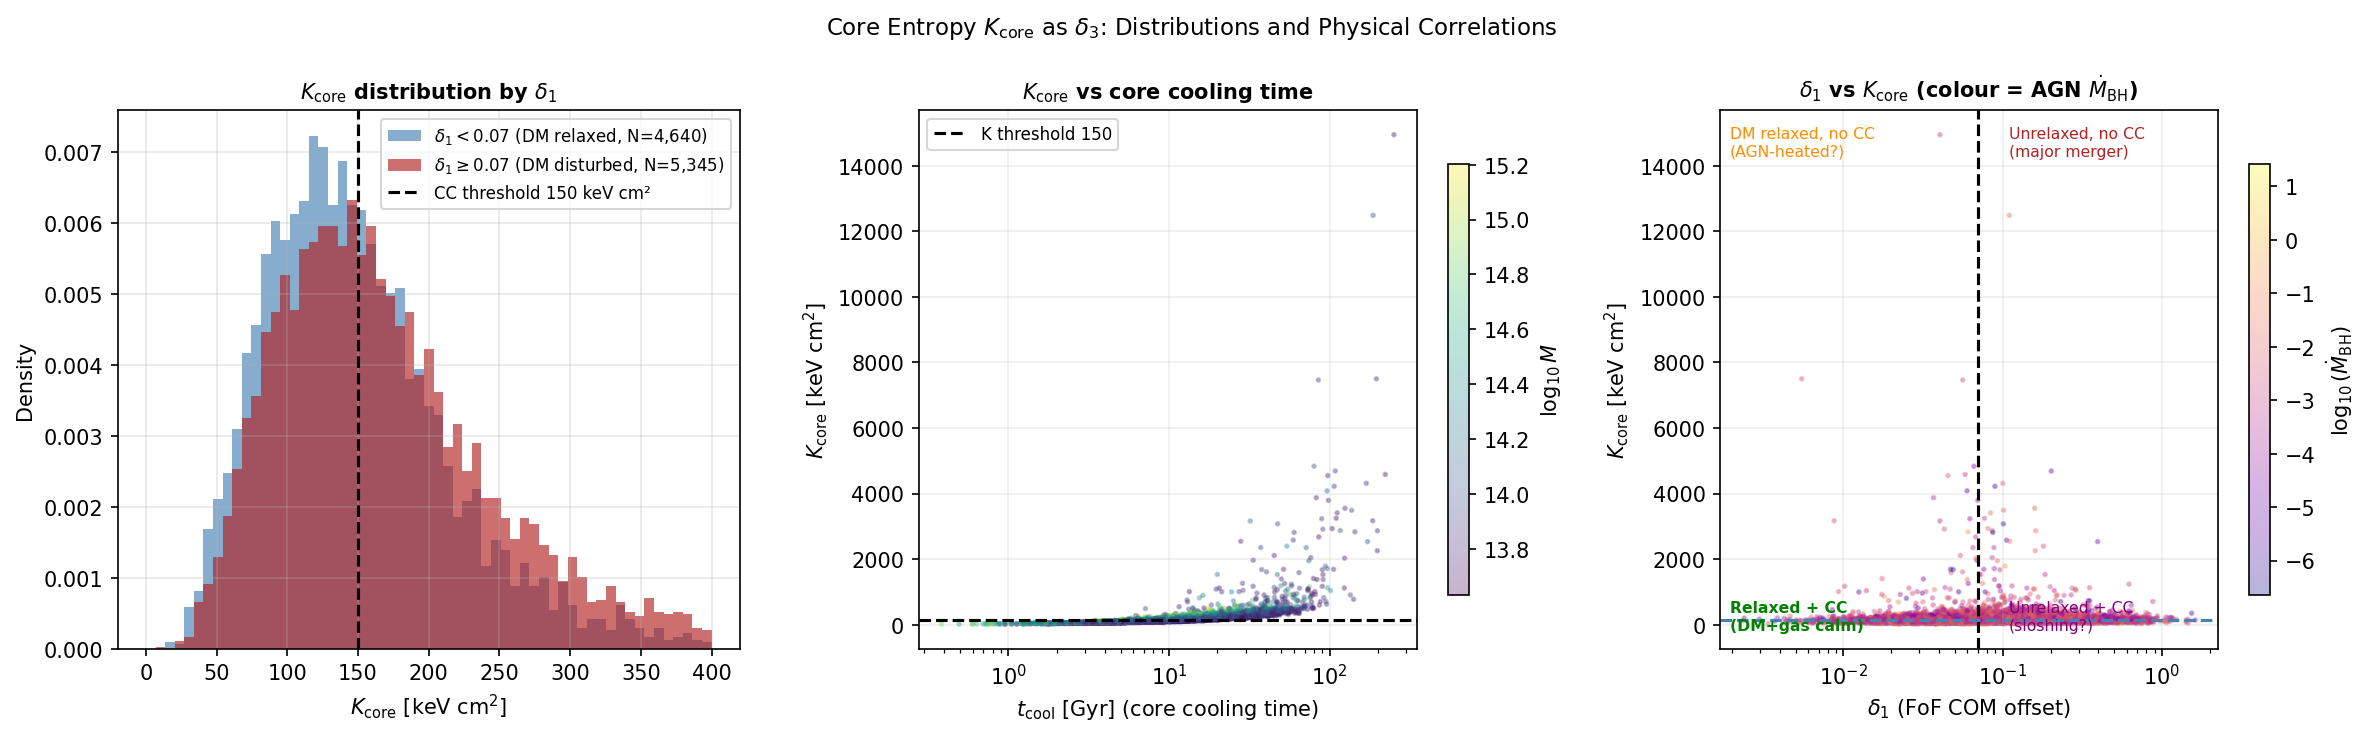
\includegraphics[width=\textwidth]{phase5_core_entropy_analysis.png}
  \caption{Core thermodynamic properties across the sample.
    \emph{Top left:} $\Kcore$ distribution for DM-relaxed (R1, blue) and DM-disturbed
    ($\lnot$R1, orange) populations.  \emph{Top right:} AGN black hole accretion rate
    vs.\ $\Kcore$, showing enhanced AGN activity in high-entropy halos consistent with
    recent feedback heating.  \emph{Bottom left:} Core cooling time vs.\ $\Kcore$,
    confirming the expected anti-correlation ($t_{\rm cool} \propto K^{3/2}$).
    \emph{Bottom right:} $\Kcore$ vs.\ halo mass, showing no strong mass trend,
    confirming the mass-independence of the cool-core classification at these masses.}
  \label{fig:kcore}
\end{figure*}

Figure~\ref{fig:kcore} shows core thermodynamic properties across the full sample.

The $\Kcore$ distributions for DM-relaxed (R1) and DM-disturbed ($\lnot$R1) halos
(top left) are clearly offset: DM-disturbed halos have a higher fraction of elevated
core entropy, but the distributions overlap substantially, again demonstrating that DM
structural state and core thermodynamic state are not strongly coupled.
The anti-correlation between $\Kcore$ and core cooling time (bottom left) provides
a fundamental validation: lower-entropy gas radiates more efficiently, yielding shorter
cooling times as expected from the self-similar scaling $t_{\rm cool} \propto K^{3/2}$
\citep{voit2005}.

The absence of a strong $\Kcore$--$M_{500c}$ trend (bottom right) confirms that the
cool-core classification is not mass-dependent over the range sampled here.
Cool-core formation is governed by core cooling efficiency rather than total cluster
mass \citep{burns2008}, so the 50\% cool-core fraction is approximately uniform across
the mass range $5\times10^{13}$--$10^{15}\,h^{-1}\Msun$.

Notably, the AGN black hole accretion rate (BHR) is elevated in the high-$\Kcore$
population (top right).  This runs in the expected direction for an AGN feedback cycle:
when feedback heats the core, entropy rises, cooling is suppressed, and eventually the
feedback quenches --- but during the active heating phase the BHR itself is elevated.
The elevated BHR in high-$\Kcore$ halos is consistent with a population of clusters
where AGN feedback has \emph{recently} been the dominant core heating mechanism,
destroying what may have been a pre-existing cool core.

\FloatBarrier
%-----------------------------------------------------------------------
\section{Extreme Unrelaxed Systems}
\label{sec:extreme}

\begin{figure*}[htbp]
  \centering
  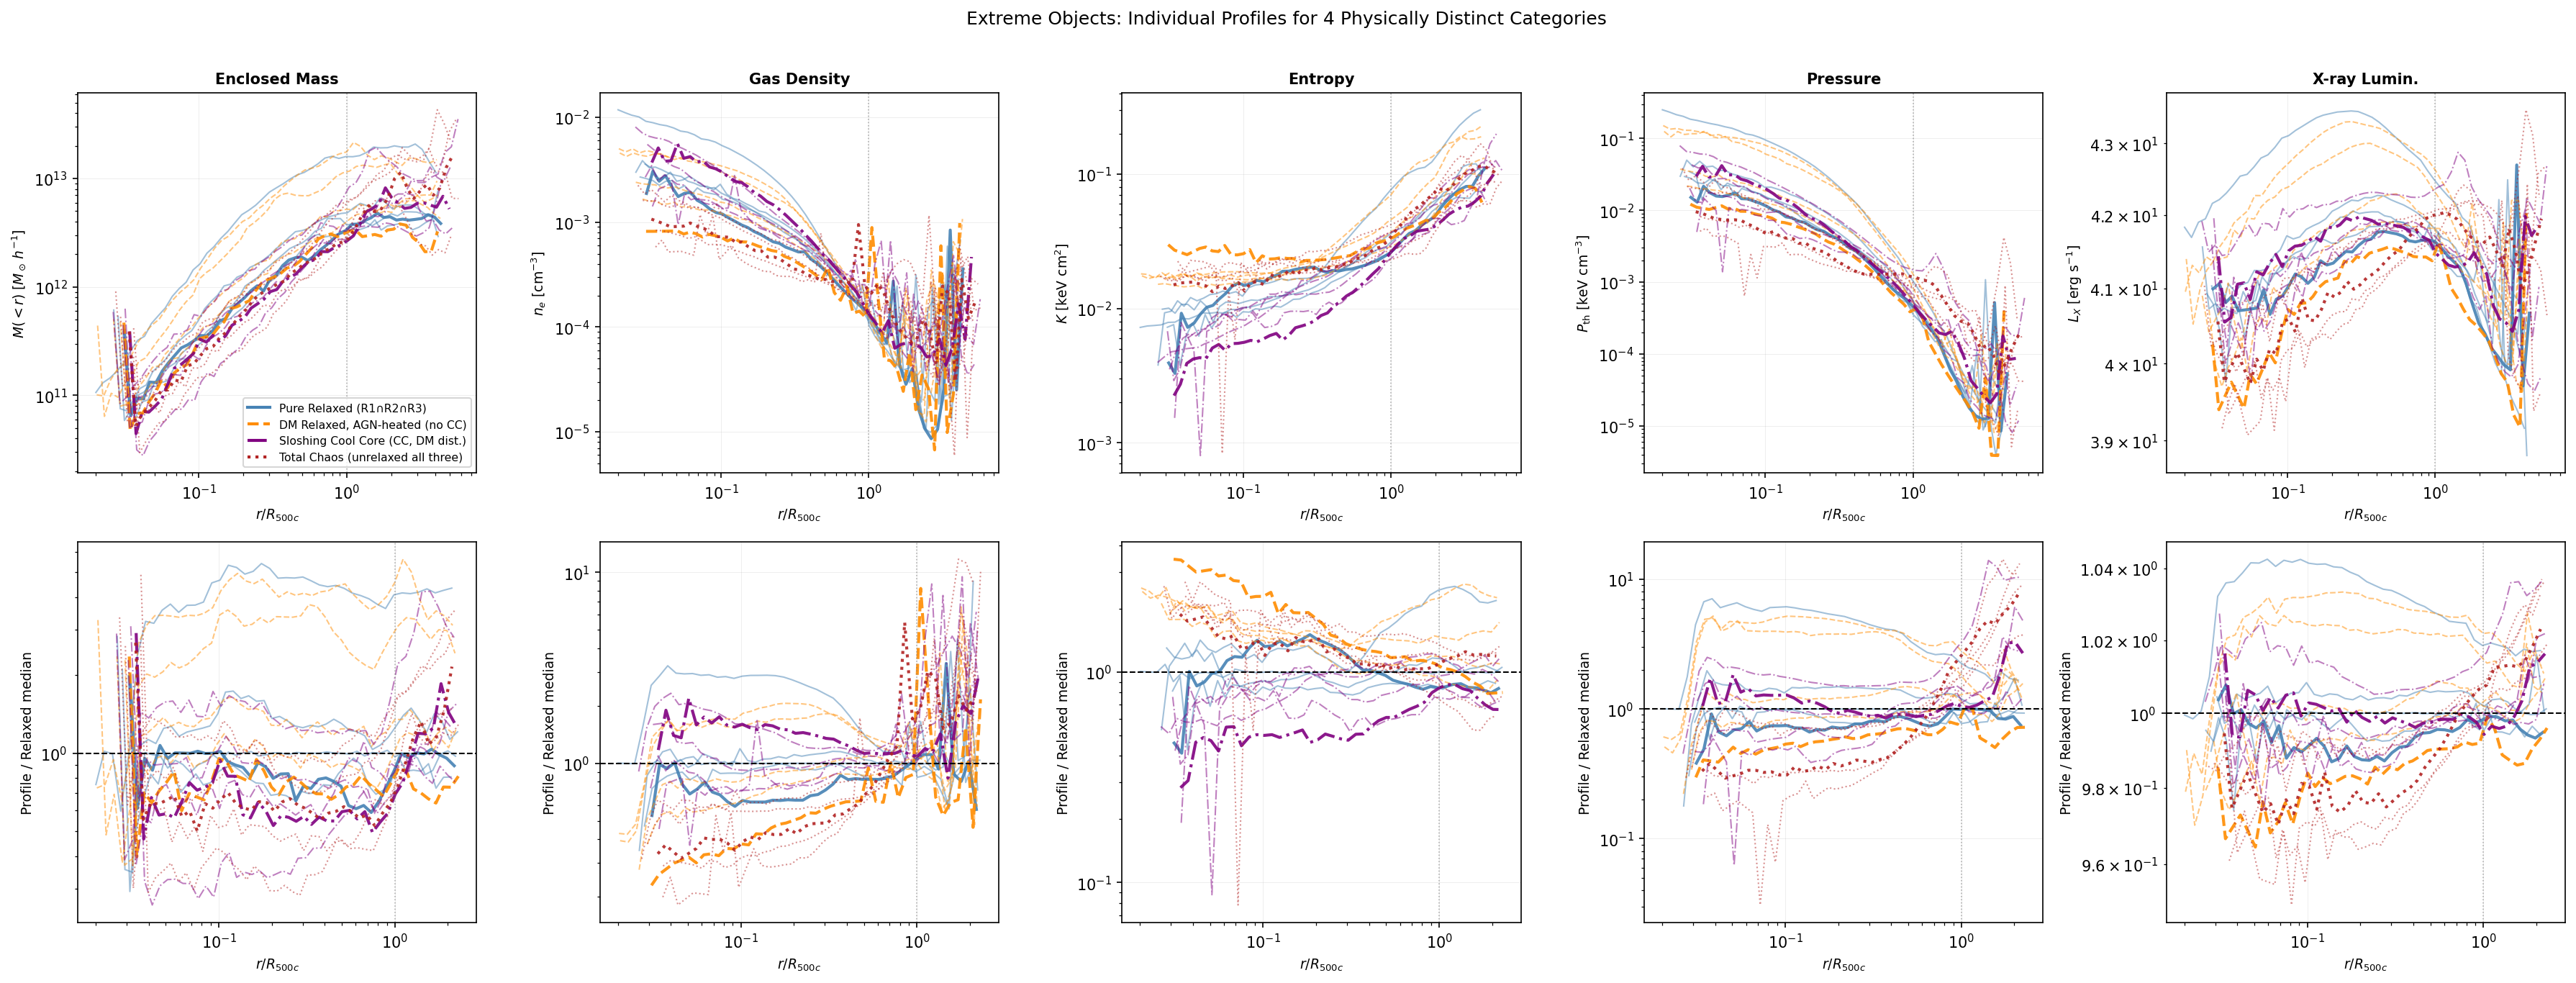
\includegraphics[width=\textwidth]{phase5_extreme_objects_profiles.png}
  \caption{Radial profiles of the most extreme (unrelaxed) clusters identified by each
    criterion: highest $\deltai$ (top row), highest $\deltaii$ (middle row), and highest
    $\Kcore$ (bottom row).  For each, profiles of electron density, entropy, and thermal
    pressure are shown alongside the full-sample stacked median (grey shaded region).
    Each extreme population displays qualitatively distinct signatures corresponding
    to different physical drivers.}
  \label{fig:extreme}
\end{figure*}

Figure~\ref{fig:extreme} shows profiles of the most extreme unrelaxed clusters by each
of the three primary criteria (the $\deltai$-extreme population demonstrates the DM
structural criterion, the others demonstrate secondary criteria).

\textit{Highest $\deltai$ (major mergers).}
These clusters display the hallmarks of ongoing major mergers: bimodal or multi-peaked
enclosed mass profiles, elevated intermediate-radius gas density ($0.2$--$0.6\,\Rfive$)
from ram-pressure gas pileup, and entropy profiles with minimal central descent.
Their pressure profiles are irregular, reflecting a system far from hydrostatic
equilibrium.

\textit{Highest $\deltaii$ (sloshing/gas displacement).}
These clusters show striking gas displacement relative to the DM potential.
The gas density peak is shifted to intermediate radii rather than centred on the cluster,
producing an off-centre pressure maximum.  These are the simulation counterparts of
observed sloshing clusters with prominent cold fronts \citep{markevitch2007}, where a
gravitational perturbation has displaced the cold core gas without destroying it.

\textit{Highest $\Kcore$ (heated cores).}
These clusters have nearly flat entropy profiles with central values
$K_0 > 300\,\kevcm$ --- more than twice the cool-core threshold.  Gas density profiles
are flat and featureless in the core, consistent with thoroughly mixed, heated gas.
These represent the most AGN-heated or most recently merger-disrupted clusters in our
sample.

The three extreme populations demonstrate that the most unrelaxed clusters by each
criterion represent qualitatively different ICM states, further motivating the
multi-criterion approach.

\FloatBarrier
%-----------------------------------------------------------------------
\section{Discussion}
\label{sec:discuss}

\subsection{Physical Scale Separation Between Criteria}

A central result of this work is the clean radial separation between the discriminating
scales of the four criteria.  The DM structural offset ($\deltai$) and the DM--gas
centroid separation ($\deltaii$) both operate at $r \gtrsim 0.3\,\Rfive$: they probe
the global and intermediate structure of the cluster, shaped by mergers and sloshing
on dynamical timescales.  The core thermodynamic criteria ($\deltaiii$ and $\deltaiv$)
operate exclusively at $r < 0.15\,\Rfive$: they trace the thermal history of the dense
central gas, shaped by the competition between radiative cooling and AGN feedback on
cooling timescales.

Because these physical scales and timescales are so different, the four criteria are
only weakly correlated (see Appendix~\ref{app:concordance}).
A cluster with a disturbed DM structure need not have a disrupted cool core (and in
fact 24\% of all halos are DM-disturbed cool-core systems), and vice versa.

\subsection{The Sloshing Cool-Core Population}

The large fraction ($\approx$24\%) of halos classified as DM-disturbed cool-core clusters
represents one of the most physically interesting results.  These systems have experienced
significant gravitational perturbations (large $\deltai$) but retain low-entropy cool
cores.  Sloshing is driven by off-axis gravitational disturbances that displace the cool
gas into a rotating motion within the gravitational potential, without fully disrupting it
\citep{markevitch2007,zuhone2010}.  Cool cores are thermally stable on timescales of
several gigayears if the cooling time is shorter than the disruption timescale
\citep{burns2008}.

In observations, sloshing cool-core clusters are identified through cold fronts --- sharp
X-ray surface brightness edges at intermediate radii.  The gas displacement captured
by $\deltaii$ provides a clean simulation-based predictor for which DM-disturbed systems
are likely to host cold fronts.  The large overlap between DM-disturbed and cool-core
classifications suggests that a pure DM morphology criterion would incorrectly classify
a quarter of all halos as unrelaxed, when in fact their thermodynamic cores are intact.

\subsection{AGN-Heated Cores}

The 18\% of halos that are DM-relaxed but lack a cool core (R1$\cap$R2$\cap\lnot$R3)
present a critical sub-population for ICM physics.  Their dynamical relaxation at large
radii rules out ongoing major mergers as the dominant heating mechanism.  The elevated
AGN BHR at high $\Kcore$ (Fig.~\ref{fig:kcore}) identifies AGN feedback as the primary
candidate: energetic outbursts from the central black hole heat the core gas, raise the
entropy above the cool-core threshold, and suppress further cooling \citep{gitti2012}.
The causal direction remains uncertain from a single snapshot --- elevated BHR could
reflect an ongoing feedback episode that is \emph{producing} the high entropy, or the
AGN may simply be accreting more efficiently from the thermally disrupted core gas.
Tracking AGN histories across cosmic time is needed to resolve this.

\subsection{Comparison with Observational Criteria}

Our simulation-based criteria have observational analogues but are not identical to any
single observational metric.  The DM COM offset $\deltai$ is most similar to the
morphological centroid shift or power ratio measured in X-ray imaging \citep{cassano2010}.
The DM--gas offset $\deltaii$ corresponds most closely to the optical/lensing-to-X-ray
centroid offset.  The core entropy $\deltaiii$ is directly measurable from X-ray
spectroscopy and surface brightness profiles \citep{hudson2010}.

The TPI criterion $\deltaiv$ is particularly relevant for future X-ray observatories
(Athena, AXIS, HUBS) that will provide spatially resolved spectroscopy for large cluster
samples.  It requires only two measurable quantities --- the core electron density
(from X-ray surface brightness) and the core-to-global temperature ratio (from
spectroscopy) --- both already accessible from existing facilities for nearby clusters.

\subsection{Simulation Caveats}

AGN feedback prescriptions in HACC are calibrated to reproduce galaxy stellar mass
functions rather than specifically the cool-core fraction; the 50\% cool-core fraction
we find is consistent with observational estimates \citep{hudson2010} but may be
sensitive to the feedback model.  The limited resolution in cluster cores ($\lesssim$ a
few kpc physical) means that the smallest-scale cooling instabilities may not be fully
resolved, making the absolute value of the $\Kcore$ threshold somewhat resolution-dependent.

\FloatBarrier
%-----------------------------------------------------------------------
\section{Conclusions}
\label{sec:conclusions}

We have analysed 9{,}985 galaxy clusters from the Frontier-E HACC hydrodynamical simulation
at $z=0$ using four complementary relaxation criteria spanning DM structural, morphological,
and thermodynamic channels.  Our main conclusions are:

\begin{enumerate}

\item \textbf{Criteria probe physically distinct radial scales.}
  The DM structural criterion ($\deltai$) and the DM--gas morphological criterion
  ($\deltaii$) discriminate at $r = 0.3$--$1.0\,\Rfive$ and $0.3$--$0.7\,\Rfive$,
  respectively, tracing merger and sloshing dynamics.  The core thermodynamic criteria
  ($\deltaiii$, $\deltaiv$) discriminate exclusively at $r < 0.15\,\Rfive$, tracing
  the thermal history of the central gas.  This clean radial separation establishes why
  the criteria are physically complementary rather than redundant.

\item \textbf{Cool-core differences are confined to the cluster core.}
  Within DM-relaxed halos, cool-core (R3) and non-cool-core ($\lnot$R3) clusters show
  diverging profiles only inside $0.15\,\Rfive$: cool-core clusters have
  $2$--$3\times$ lower central entropy, $\sim$10$\times$ higher core X-ray luminosity,
  and steeply rising central density.  Profiles converge completely at $r > 0.15\,\Rfive$,
  establishing a clean diagnostic scale for cool-core classification.

\item \textbf{DM relaxation alone is an incomplete relaxation criterion.}
  Of all halos, 24\% are DM-disturbed yet retain intact cool cores (sloshing cool-core
  candidates), while 18\% are DM-relaxed yet lack cool cores (AGN-heated or post-merger).
  A pure DM morphology criterion would misclassify both of these populations, motivating
  the use of ICM-based complementary criteria.

\item \textbf{Cool-core bias in scaling relations.}
  Cool-core clusters are elevated in $L_X$ at fixed spectroscopic temperature by up to
  a factor of $\sim$3 (cool-core luminosity bias), and show $\sim$30\% lower scatter
  in the $Y_{\rm SZ}$--$M_{500c}$ relation compared to disturbed clusters, confirming
  the importance of relaxation-state selection for precision cluster cosmology.

\item \textbf{AGN feedback is imprinted on core entropy.}
  Clusters with the highest $\Kcore$ show elevated AGN black hole accretion rates,
  consistent with recent AGN feedback as the dominant core heating mechanism in the
  DM-relaxed non-cool-core population.

\item \textbf{TPI provides finer-grained thermodynamic information.}
  The TPI criterion ($\deltaiv$) independently weights core density and core temperature
  drop, two distinct observational channels.  The 31.5\% discordance with $\deltaiii$
  (Appendix~\ref{app:tpi}) reveals physically distinct ICM states where either the
  density or the temperature drop dominates the cool-core signature, information that
  is degenerate in $\Kcore$ alone.

\end{enumerate}

These results motivate multi-criterion relaxation assessments in large X-ray and SZ
cluster surveys.  Future work will extend this analysis to the redshift evolution of
these populations and the connection between relaxation state and radio halo occurrence.

%-----------------------------------------------------------------------
\acknowledgments
The Frontier-E simulation was performed using the HACC framework.
Data access and analysis were enabled by the OpenCosmo data platform and Globus Flows
infrastructure.

%-----------------------------------------------------------------------
\bibliography{relaxation_criteria}

%-----------------------------------------------------------------------
\appendix

\section{Population Cross-Classification Statistics}
\label{app:concordance}

\begin{figure*}[htbp]
  \centering
  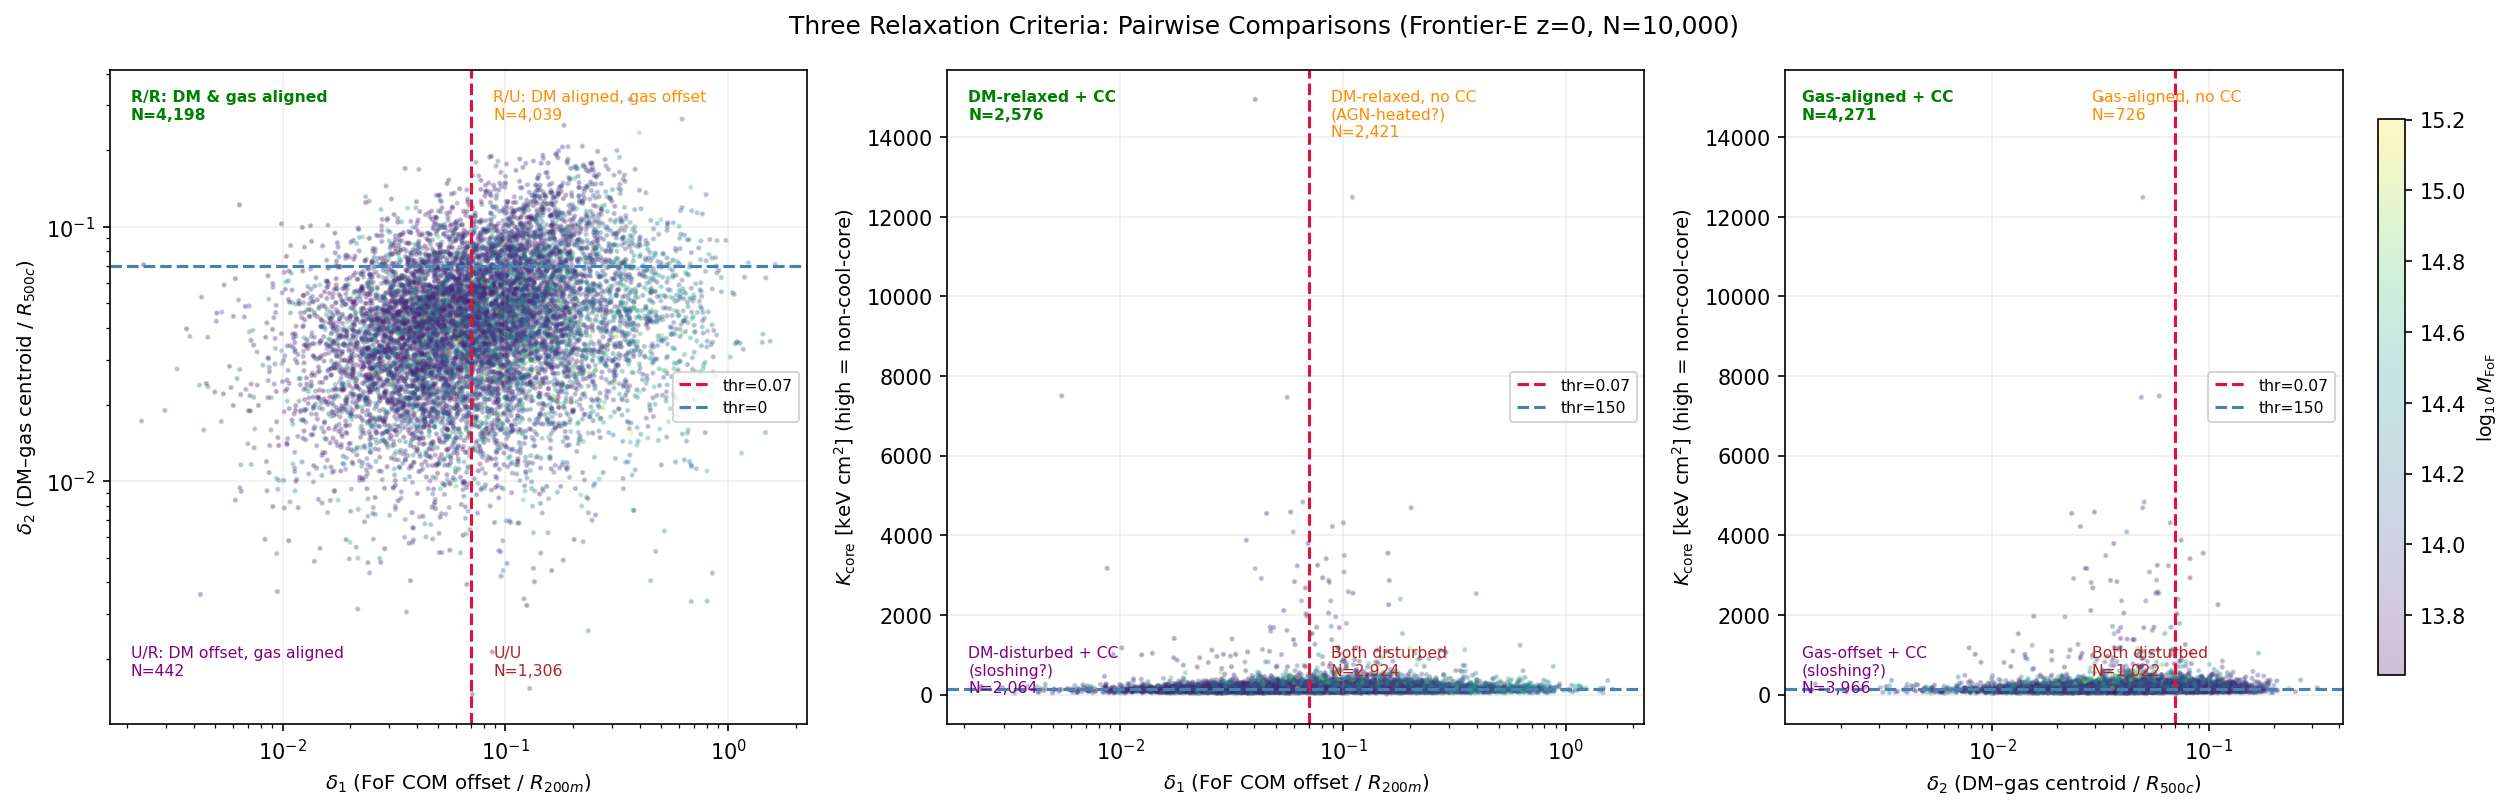
\includegraphics[width=0.90\textwidth]{phase5_three_criteria_comparison.png}
  \caption{Distributions and cross-comparisons of the three primary scalar criteria
    ($\deltai$, $\deltaii$, $\deltaiii$) for all 9{,}985 halos.
    \emph{Top row:} Histograms with vertical dashed lines at the relaxation thresholds.
    \emph{Lower panels:} Pairwise scatter plots colour-coded by a third criterion.
    The limited pairwise correlation confirms that each criterion captures an independent
    dimension of relaxation state.  The ``sloshing cool-core'' population
    ($\Kcore < 150\,\kevcm$, large $\deltai$) is clearly visible in the upper-left
    region of the $\deltai$--$\Kcore$ panel.}
  \label{fig:criteria}
\end{figure*}

Figure~\ref{fig:criteria} shows the distributions and pairwise scatter of the three
primary criteria.  The limited correlations visible in the pairwise panels are the key
demonstration that each criterion captures a distinct dimension of cluster relaxation
state.  In particular, $\deltai$ and $\Kcore$ are only weakly anti-correlated: more
disturbed DM structures do \emph{not} automatically imply higher core entropy.

Table~\ref{tab:populations} summarises the concordance statistics for the three primary
criteria, and for the core thermodynamic concordance between $\deltaiii$ and $\deltaiv$.

\begin{table}[htbp]
\centering
\caption{Population cross-classification statistics ($N_{\rm total}=9{,}985$).
  Abbreviations: R1 $\equiv \deltai<0.07$; R2 $\equiv \deltaii<0.07$;
  R3 $\equiv \Kcore < 150\,\kevcm$; R4 $\equiv \TPI > 0$.}
\label{tab:populations}
\begin{tabular}{lrr}
\toprule
Population & $N$ & Fraction \\
\midrule
\multicolumn{3}{l}{\textit{Single-criterion fractions:}} \\
DM-relaxed (R1)            & 4{,}640 & 46.5\% \\
Cool-core (R3)             & 4{,}997 & 50.0\% \\
Cool-core by TPI (R4)      & 5{,}344 & 53.5\% \\[3pt]
\multicolumn{3}{l}{\textit{R2 within DM-relaxed halos (R1):}} \\
R1$\cap$R2 (gas-coherent)  & 4{,}198 & 90.5\% of R1 \\
R1$\cap\lnot$R2 (gas-displaced) & 442 & 9.5\% of R1 \\[3pt]
\multicolumn{3}{l}{\textit{Three-criterion concordant populations:}} \\
Concordant Relaxed (R1$\cap$R2$\cap$R3) & 2{,}398 & 24.0\% \\
Concordant Disturbed ($\lnot$R1$\cap\lnot$R2$\cap\lnot$R3) & 758 & 7.6\% \\
DM-disturbed cool-core ($\lnot$R1$\cap$R3) & 2{,}421 & 24.2\% \\
DM-relaxed, no cool-core (R1$\cap$R2$\cap\lnot$R3) & 1{,}800 & 18.0\% \\[3pt]
\multicolumn{3}{l}{\textit{Core thermodynamic concordance ($\deltaiii$ vs.\ $\deltaiv$):}} \\
Both CC ($\Kcore<150$ and $\TPI>0$)         & 3{,}598 & 36.0\% \\
Both NCC ($\Kcore>150$ and $\TPI \le 0$)    & 3{,}242 & 32.5\% \\
$\Kcore$-CC only (high $n_e$, no T-drop)    & 1{,}399 & 14.0\% \\
TPI-CC only (T-drop, moderate $n_e$)        & 1{,}746 & 17.5\% \\
\bottomrule
\end{tabular}
\end{table}

The four key concordant populations identified from three-criterion cross-classification are:

\textbf{Concordant Relaxed (24.0\%).}
Halos satisfying all three primary criteria simultaneously (smooth DM structure, coherent
DM--gas morphology, low-entropy cool core).  These represent the classical relaxed,
cool-core cluster and likely host the most reliable hydrostatic mass estimates.

\textbf{Concordant Disturbed (7.6\%).}
Halos failing all three criteria.  They are experiencing major mergers, with disturbed DM,
asymmetric gas, and elevated core entropy.  These correspond to the non-cool-core clusters
found in X-ray surveys \citep{hudson2010,burns2008}, commonly associated with diffuse
radio emission \citep{cassano2010}.

\textbf{DM-disturbed Cool-Core (24.2\%).}
Halos with disturbed DM ($\deltai \geq 0.07$) but intact cool cores ($\Kcore < 150\,\kevcm$).
These are strong candidates for \emph{sloshing cool-core clusters}: large-scale DM
substructure indicates a recent interaction, yet the cool core has survived
\citep{markevitch2007,zuhone2010}.  The 24\% fraction is consistent with the long
survival time of cool cores against moderate dynamical disturbances \citep{burns2008}.

\textbf{DM-Relaxed, No Cool Core (18.0\%).}
Dynamically settled halos at large radii (R1 and R2) with elevated core entropy.
Their cool cores have been destroyed or suppressed, most likely by AGN feedback
\citep{gitti2012}.

\begin{figure*}[htbp]
  \centering
  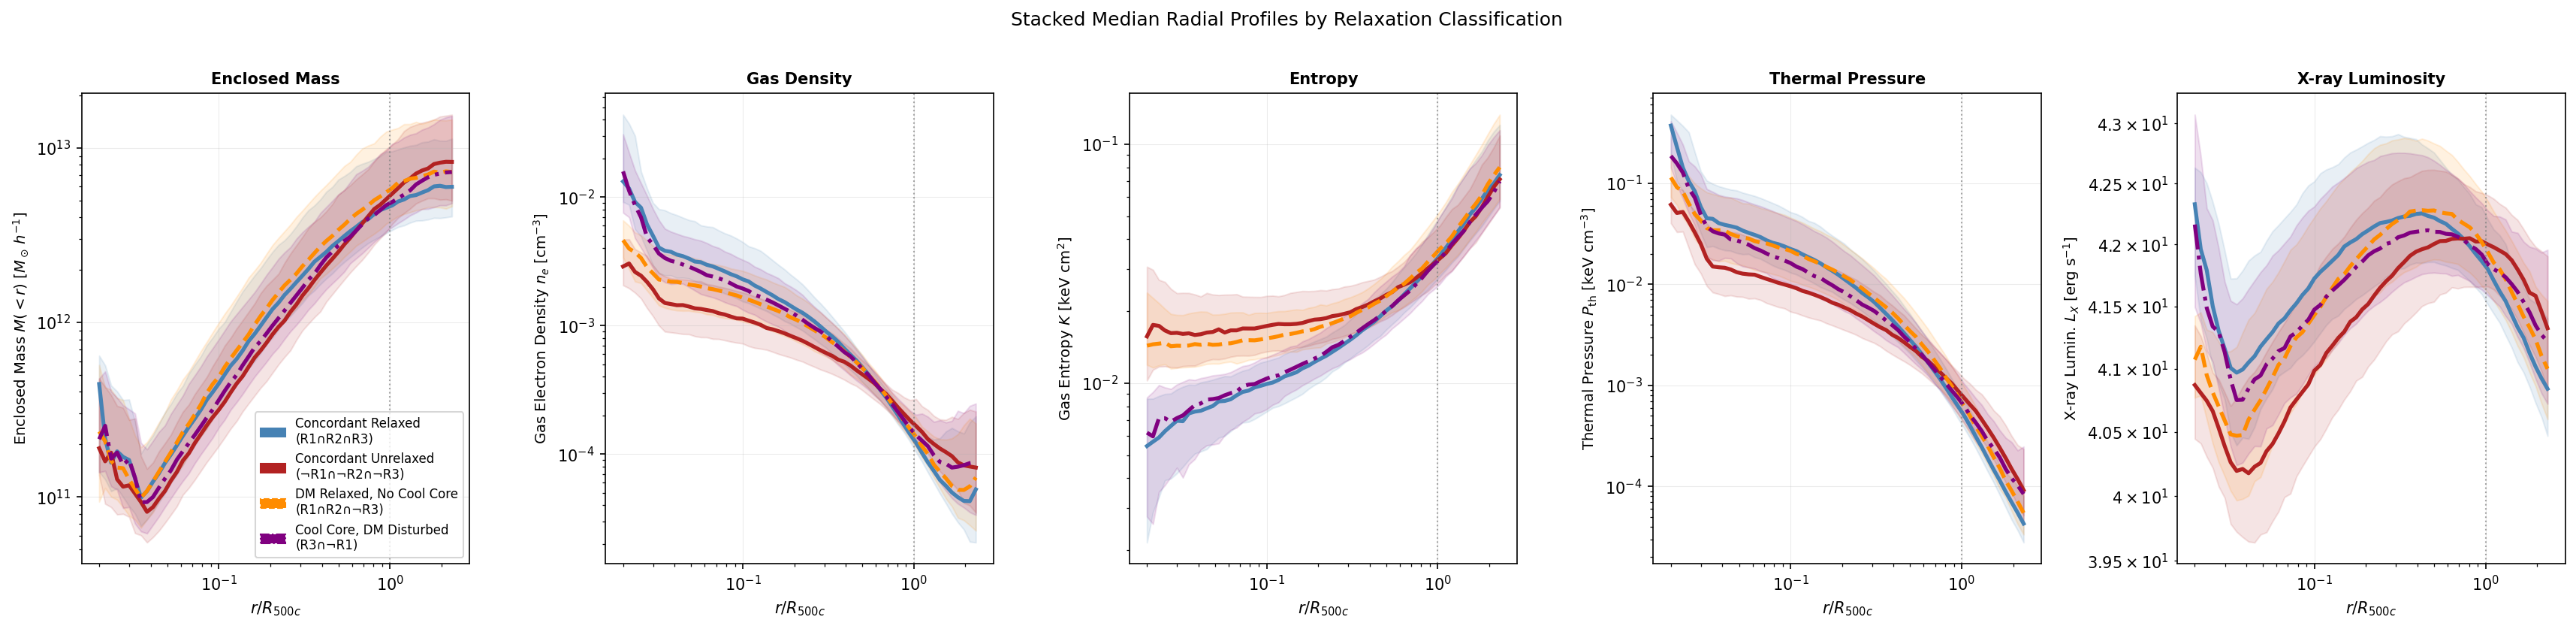
\includegraphics[width=\textwidth]{phase5_stacked_profiles_by_class.png}
  \caption{Stacked median profiles for the four concordant population classes:
    concordant relaxed (CR), DM-disturbed cool-core (DC), DM-relaxed no cool-core (RN),
    and concordant disturbed (CD).
    Profiles shown are gas electron density, specific entropy, thermal pressure, and
    bolometric X-ray luminosity.  The CR population shows the canonical cool-core shape,
    while CD clusters have flat, high-entropy profiles.  Notably, the DC profiles
    closely match CR profiles at $r < 0.2\,\Rfive$, confirming that the DM disturbance
    in the DC population has not propagated into the cool core.}
  \label{fig:stacked_app}
\end{figure*}

Figure~\ref{fig:stacked_app} shows stacked median profiles for all four concordant
populations.  The DM-disturbed cool-core (DC) profiles closely track the concordant
relaxed (CR) profiles in the core ($r < 0.2\,\Rfive$), diverging only at intermediate and
large radii where the DM disturbance manifests.  This demonstrates that $\deltai$ and
$\deltaiii$ are functionally orthogonal: DM structural disturbance does not automatically
disrupt the cool core.

%-----------------------------------------------------------------------
\section{TPI Diagnostic and \texorpdfstring{$\deltaiii$--$\deltaiv$}{delta3-delta4} Discordance}
\label{app:tpi}

\begin{figure*}[htbp]
  \centering
  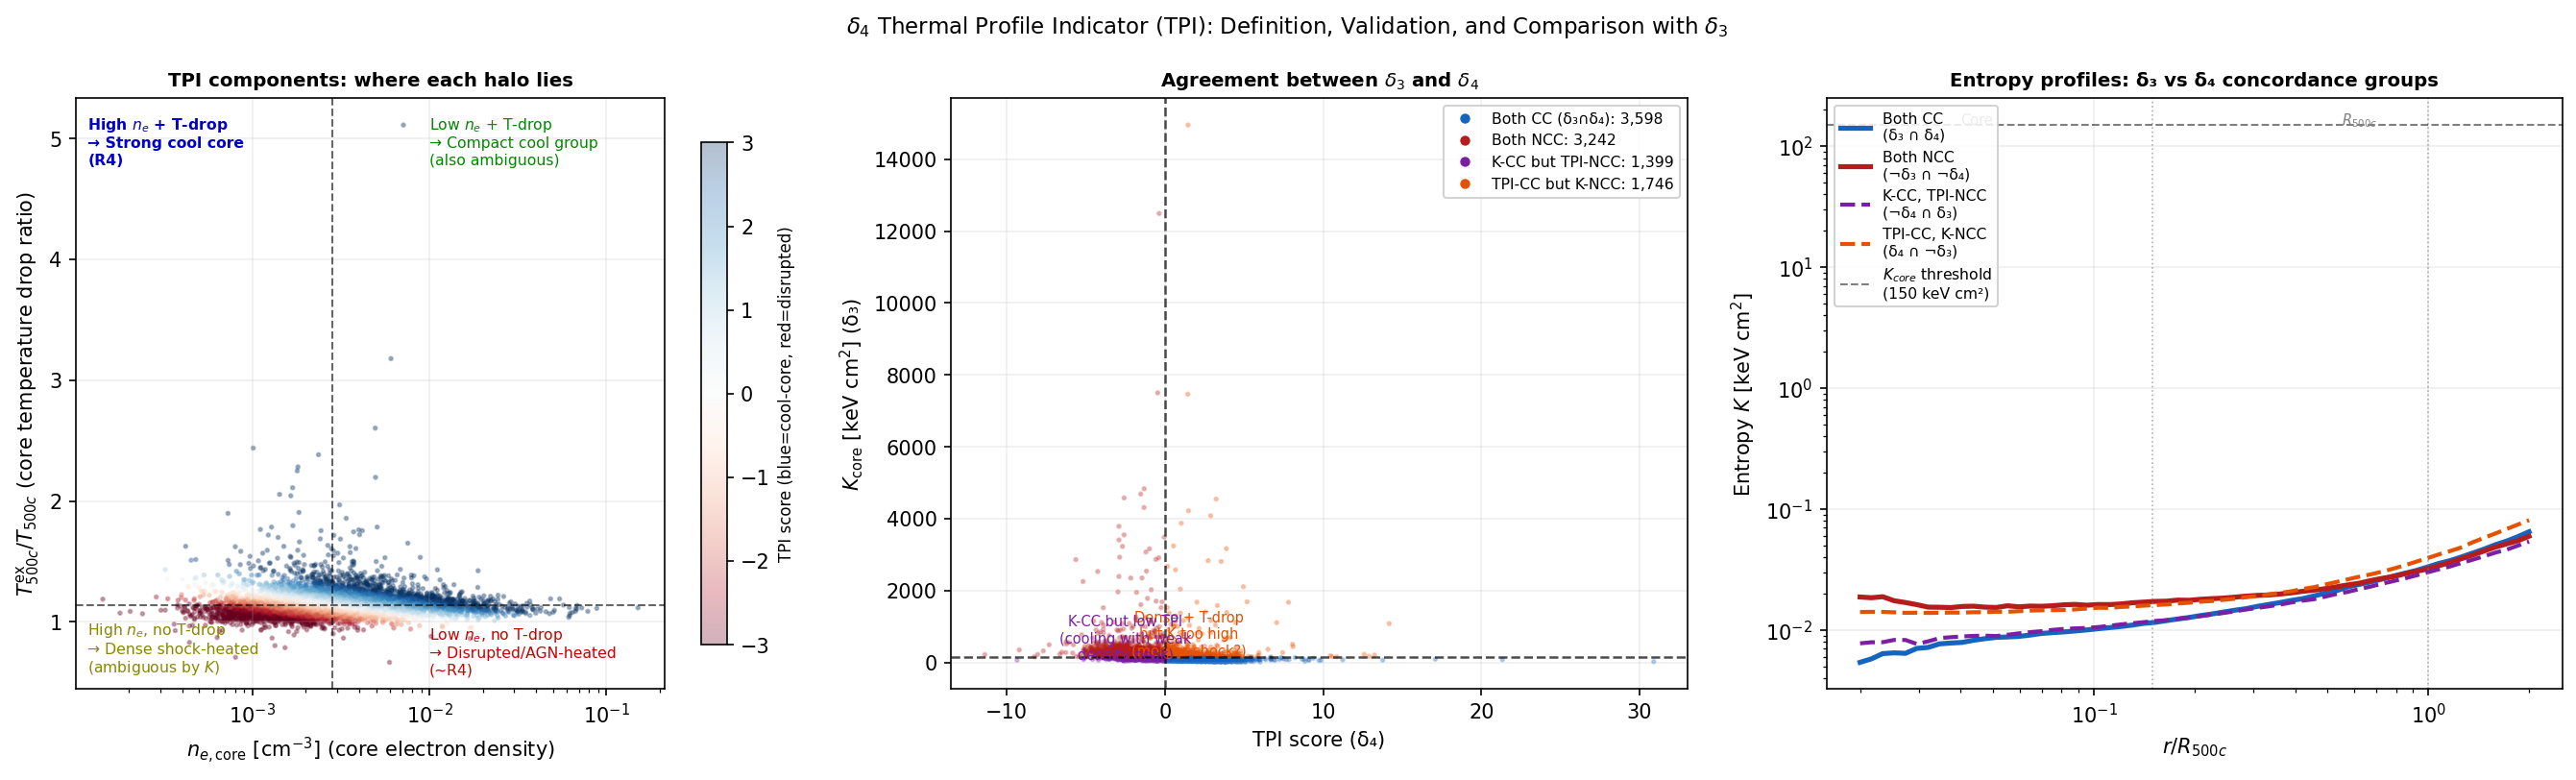
\includegraphics[width=0.95\textwidth]{phase6_tpi_diagnostic.png}
  \caption{TPI diagnostic plots.
    \emph{Left:} Core electron density $n_{e,\rm core}$ vs.\ temperature ratio
    $T_{\rm BoloEx}/T_{500c}$, colour-coded by TPI value.  Dashed lines indicate the
    sample medians; halos in the upper-right quadrant (above both medians) are classified
    as cool-core by TPI.  \emph{Centre:} TPI vs.\ $\Kcore$, revealing the four
    $\deltaiii$--$\deltaiv$ concordant and discordant populations.
    \emph{Right:} Stacked entropy profiles for the four concordance groups, showing
    their distinct thermodynamic structures.}
  \label{fig:tpi}
\end{figure*}

Figure~\ref{fig:tpi} illustrates the origin of the 31.5\% discordance between $\deltaiii$
and $\deltaiv$ (see also Table~\ref{tab:populations}).

The left panel shows the $n_{e,\rm core}$--$T_{\rm BoloEx}/T_{500c}$ plane, which
forms the natural basis for TPI.  The 1{,}399 halos that are $\Kcore$-cool-core but
not TPI-cool-core (high density, modest temperature ratio) have high electron density
without a corresponding temperature drop.  These may be systems where gas compression
from a recent minor merger or sloshing episode temporarily elevated the density while the
temperature equilibration is incomplete, or where AGN heating prevents the temperature
from dropping despite the density concentration.

Conversely, the 1{,}746 TPI-cool-core clusters that do not satisfy $\deltaiii$ (moderate
density, strong temperature drop) have a spectroscopic temperature decrease without
sufficient density to produce low $K = Tn^{-2/3}$.  Their core entropy exceeds
150\,$\kevcm$ despite the temperature drop because the electron density is insufficiently
high.  These may represent systems in the early stages of cool-core formation, or clusters
with an intermediate thermal state following an AGN heating episode.

The right panel confirms that these discordant populations have distinct entropy profile
shapes intermediate between the concordant cool-core and non-cool-core populations,
consistent with physically different ICM states rather than mere classification artefacts.

%-----------------------------------------------------------------------
\section{Extended Particle Morphology Panels}
\label{app:morphology}

Figures~\ref{fig:mf_R1}--\ref{fig:mf_R1notR4} show particle projections for six randomly
selected halos from each relaxation sub-class (dark matter, stars, gas mass, gas
temperature from left to right).  These complement the rank-1 gallery in
Figure~\ref{fig:gallery} by sampling a broader range of morphologies within each group.

\begin{figure*}[htbp]
  \centering
  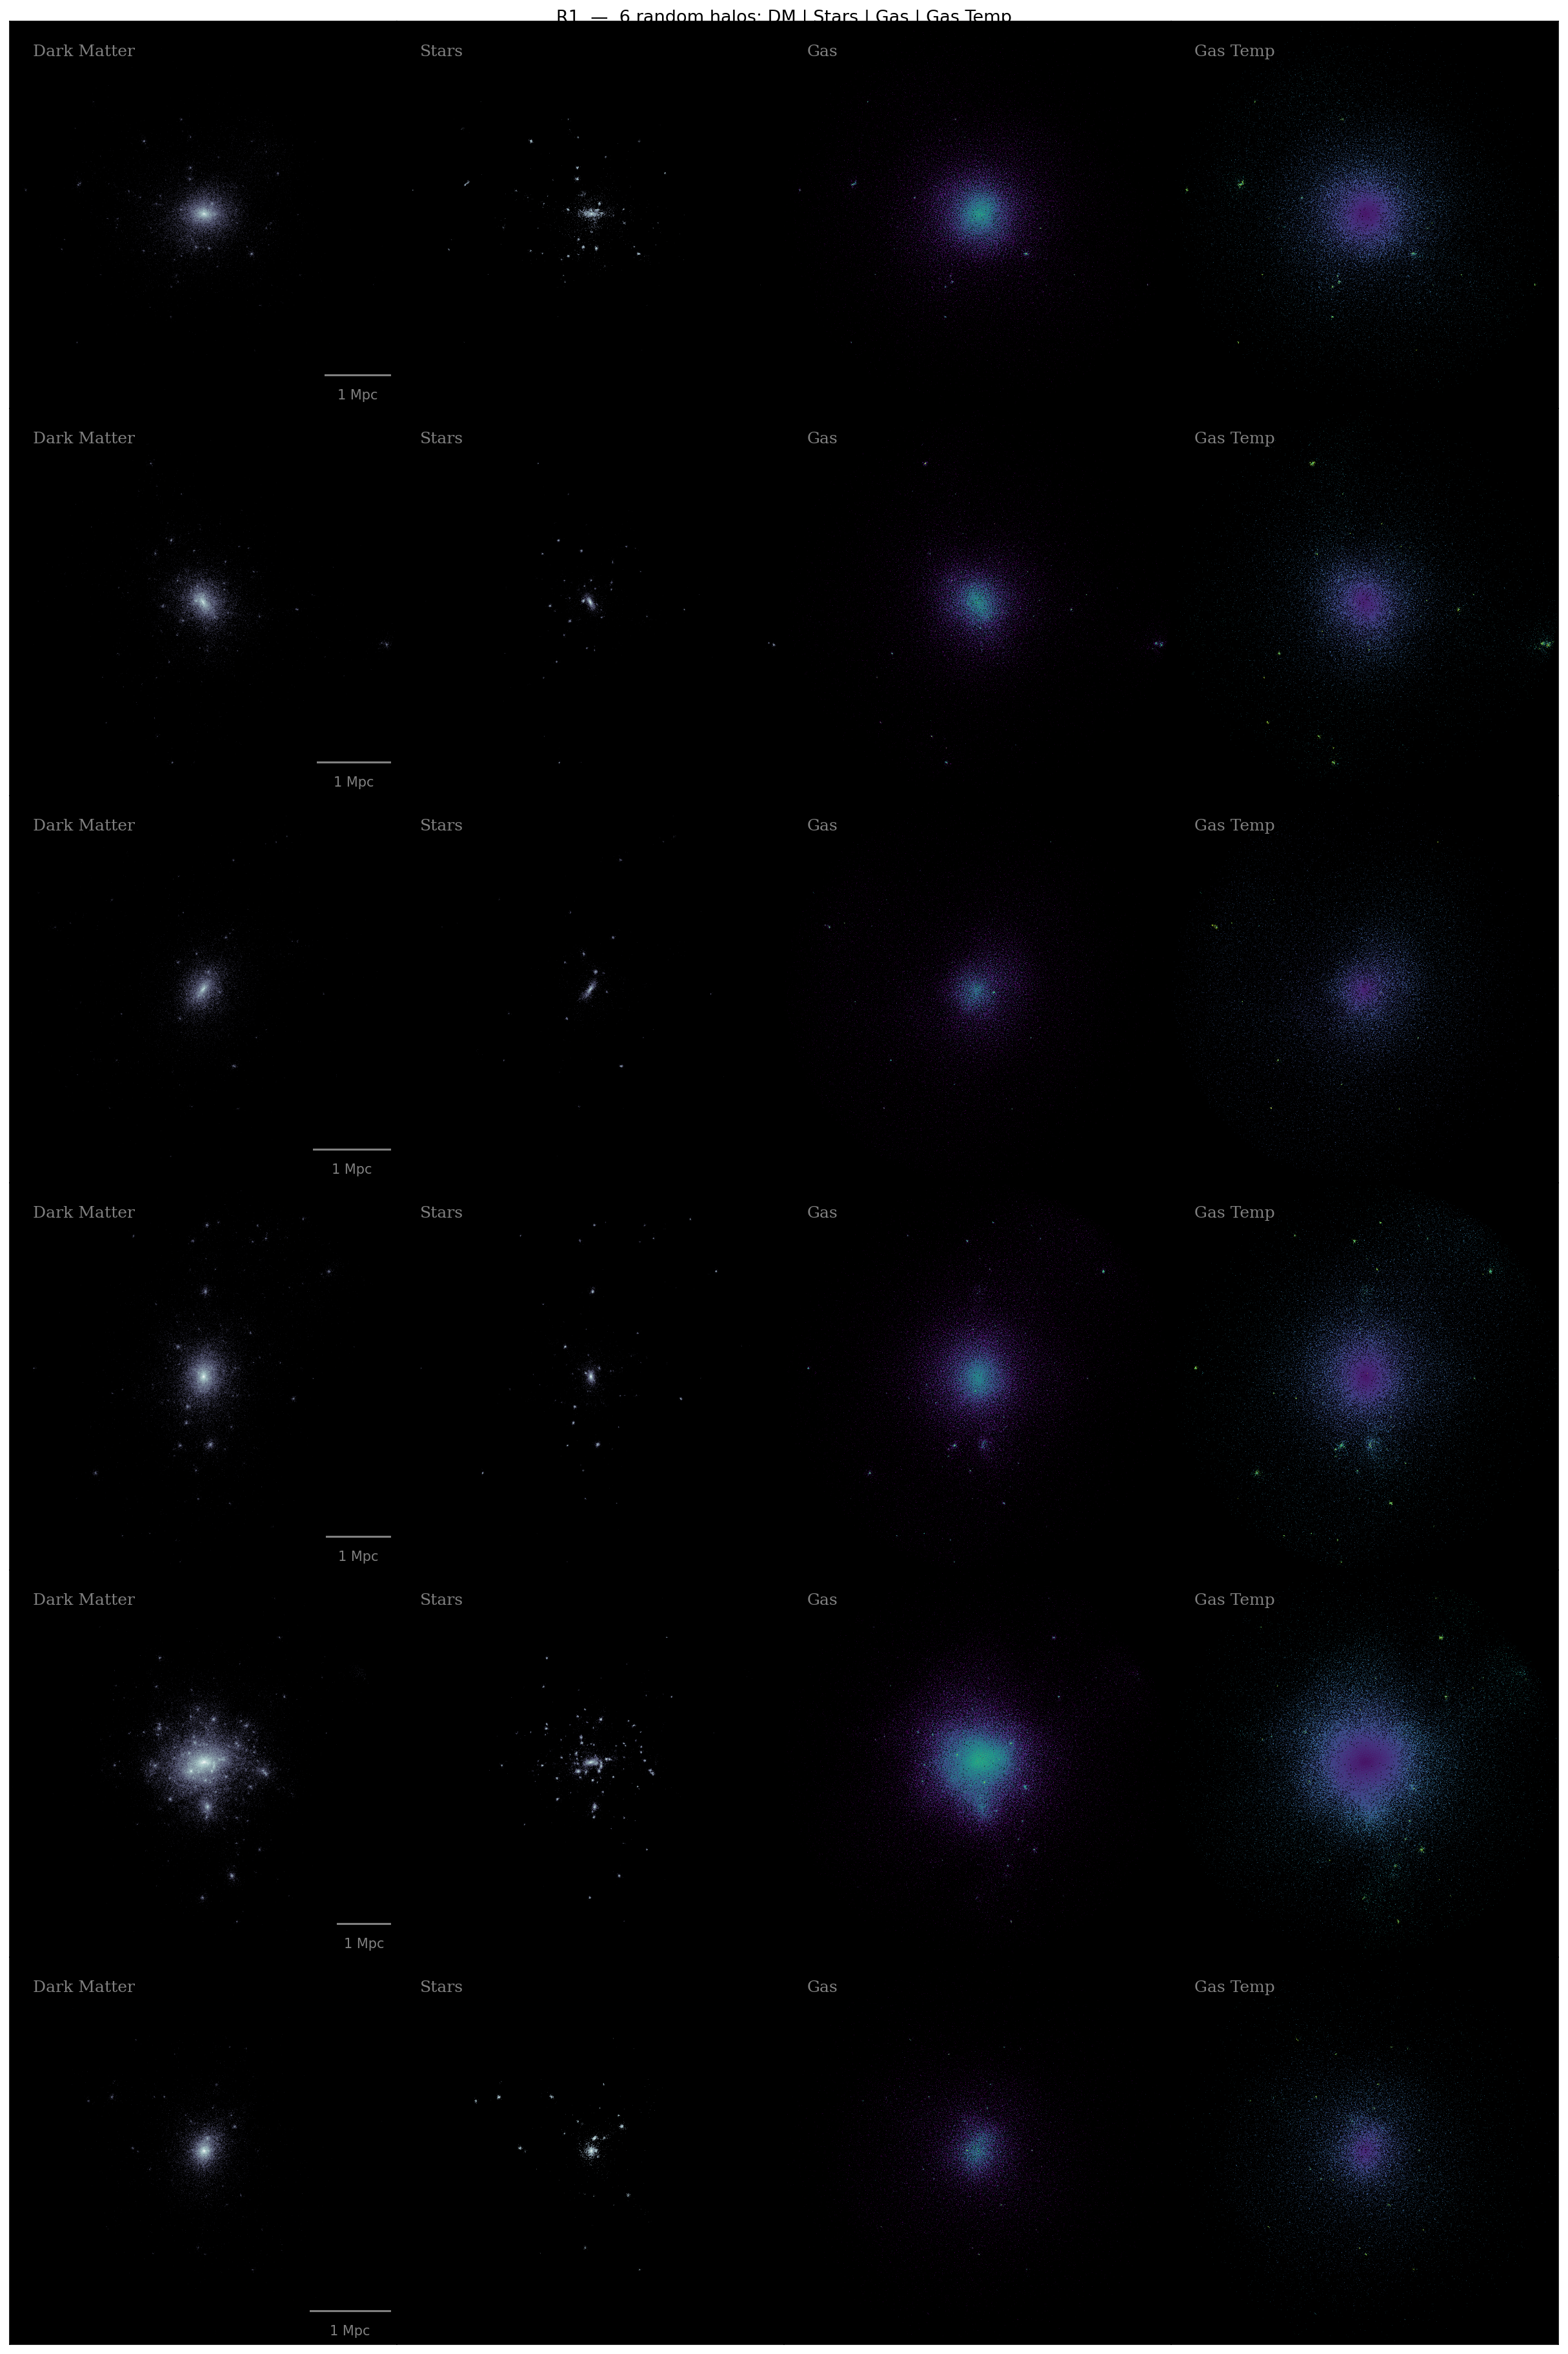
\includegraphics[width=\textwidth]{halo_viz/R1/multifield_4field_random6.png}
  \caption{Six randomly selected R1 halos (DM-relaxed baseline, $\deltai < 0.07$).
    Each row is one halo; columns show dark matter mass, stellar mass, gas mass, and
    gas temperature.}
  \label{fig:mf_R1}
\end{figure*}

\begin{figure*}[htbp]
  \centering
  
\includegraphics[width=\textwidth]{halo_viz/R1_andR2/multifield_4field_random6.png}
  \caption{Six randomly selected R1$\cap$R2 halos (gas-coherent, $\deltaii < 0.07$).}
  \label{fig:mf_R1andR2}
\end{figure*}

\begin{figure*}[htbp]
  \centering
  
\includegraphics[width=\textwidth]{halo_viz/R1_notR2/multifield_4field_random6.png}
  \caption{Six randomly selected R1$\cap\lnot$R2 halos (gas-displaced, $\deltaii \geq 0.07$).
    Note the visually offset gas centroid relative to the DM halo in several examples.}
  \label{fig:mf_R1notR2}
\end{figure*}

\begin{figure*}[htbp]
  \centering
  
\includegraphics[width=\textwidth]{halo_viz/R1_andR3/multifield_4field_random6.png}
  \caption{Six randomly selected R1$\cap$R3 halos (cool-core, $\Kcore < 150\,\kevcm$).
    Compact, bright gas concentrations and central temperature inversions are evident.}
  \label{fig:mf_R1andR3}
\end{figure*}

\begin{figure*}[htbp]
  \centering
  
\includegraphics[width=\textwidth]{halo_viz/R1_notR3/multifield_4field_random6.png}
  \caption{Six randomly selected R1$\cap\lnot$R3 halos (non-cool-core, $\Kcore \geq 150\,\kevcm$).
    Gas distributions are more diffuse with uniformly warm cores.}
  \label{fig:mf_R1notR3}
\end{figure*}

\begin{figure*}[htbp]
  \centering
  
\includegraphics[width=\textwidth]{halo_viz/R1_andR4/multifield_4field_random6.png}
  \caption{Six randomly selected R1$\cap$R4 halos (TPI cool-core, TPI $> 0$).}
  \label{fig:mf_R1andR4}
\end{figure*}

\begin{figure*}[htbp]
  \centering
  
\includegraphics[width=\textwidth]{halo_viz/R1_notR4/multifield_4field_random6.png}
  \caption{Six randomly selected R1$\cap\lnot$R4 halos (TPI non-cool-core, TPI $\leq 0$).}
  \label{fig:mf_R1notR4}
\end{figure*}

\end{document}
